\documentclass[11pt,a4paper]{article}

% ---------------------------------------------------------------
% Packages
% ---------------------------------------------------------------
\usepackage[utf8]{inputenc}
\usepackage[T1]{fontenc}
\usepackage[french]{babel}
\usepackage{lmodern}
\usepackage{geometry}
\geometry{margin=2.5cm}
\usepackage{graphicx}
\usepackage{float}
\usepackage{hyperref}
\usepackage{xcolor}
\usepackage{listings}
\usepackage{booktabs}
\usepackage{array}
\usepackage{tabularx}
\usepackage{enumitem}
\usepackage{amsmath,amssymb}
\usepackage{caption}
\usepackage{subcaption}
\usepackage{fancyhdr}
\setlength{\headheight}{14pt}
\usepackage{titling}

% Diagramme de Gantt (à activer si pgfgantt est installé)
\usepackage{pgfgantt}
\usepackage{tikz}
\usetikzlibrary{positioning,arrows.meta}

% ---------------------------------------------------------------
% Hyperliens
% ---------------------------------------------------------------
\hypersetup{
    colorlinks=true,
    linkcolor=black,
    urlcolor=blue,
    citecolor=black
}

% ---------------------------------------------------------------
% Style code
% ---------------------------------------------------------------
\definecolor{codegray}{rgb}{0.95,0.95,0.95}
\definecolor{codekw}{rgb}{0.13,0.29,0.53}
\definecolor{codestr}{rgb}{0.45,0.45,0.45}
\definecolor{codecmt}{rgb}{0.25,0.50,0.25}

\lstset{
    backgroundcolor=\color{codegray},
    basicstyle=\ttfamily\footnotesize,
    keywordstyle=\color{codekw}\bfseries,
    stringstyle=\color{codestr},
    commentstyle=\color{codecmt}\itshape,
    breaklines=true,
    frame=single,
    showstringspaces=false,
    tabsize=2,
    captionpos=b,
    extendedchars=true,
    inputencoding=utf8,
    literate=%
        {é}{{\'e}}1 {è}{{\`e}}1 {ê}{{\^e}}1 {ë}{{\"e}}1
        {É}{{\'E}}1 {È}{{\`E}}1 {Ê}{{\^E}}1 {Ë}{{\"E}}1
        {à}{{\`a}}1 {â}{{\^a}}1 {ä}{{\"a}}1
        {À}{{\`A}}1 {Â}{{\^A}}1 {Ä}{{\"A}}1
        {î}{{\^i}}1 {ï}{{\"i}}1 {Î}{{\^I}}1 {Ï}{{\"I}}1
        {ô}{{\^o}}1 {ö}{{\"o}}1 {Ô}{{\^O}}1 {Ö}{{\"O}}1
        {û}{{\^u}}1 {ü}{{\"u}}1 {ù}{{\`u}}1
        {Û}{{\^U}}1 {Ü}{{\"U}}1 {Ù}{{\`U}}1
        {ç}{{\c c}}1 {Ç}{{\c C}}1
        {œ}{{\oe}}1 {Œ}{{\OE}}1
        {æ}{{\ae}}1 {Æ}{{\AE}}1
}

% ---------------------------------------------------------------
% En-têtes
% ---------------------------------------------------------------
\pagestyle{fancy}
\fancyhf{}
\fancyhead[L]{Système de Market Making par Apprentissage par Renforcement -- PFA}
\fancyhead[R]{\thepage}
\renewcommand{\headrulewidth}{0.4pt}

% ---------------------------------------------------------------
% Page de titre
% ---------------------------------------------------------------
\title{
    \vspace{-1cm}
    \Huge \textbf{Système de Market Making par Apprentissage par Renforcement} \\[0.5cm]
    \large PFA 2025--2026 -- ENSEIRB-MATMECA
}
\author{
    Bella Taleb El Alem \and
    Yani Haouchine \and
    Ihab Jaouad \and
    Anas Benbaki \and
    Mohamed Aziz Migaou \and
    Soufiane Sbai
}
\date{\today}

% ===============================================================
\begin{document}
% ===============================================================

\begin{titlingpage}
    \begin{center}
        \vspace*{1cm}
        {\large ENSEIRB-MATMECA} \\[0.2cm]
        {\large Filière Informatique -- 2\textsuperscript{ème} année} \\[0.2cm]
        {\large Année universitaire 2025--2026}

        \vspace{2cm}
        \rule{\textwidth}{0.5pt} \\[0.4cm]
        {\Huge \textbf{Système de Market Making}} \\[0.3cm]
        {\Huge \textbf{par Apprentissage par Renforcement}} \\[0.4cm]
        \rule{\textwidth}{0.5pt}

        \vspace{1cm}
        {\large PFA 2025--2026 -- ENSEIRB-MATMECA}

        \vfill

        {\large \textbf{Équipe :}} \\[0.4cm]
        {\large
            Bella Taleb El Alem \quad Yani Haouchine \quad Ihab Jaouad \\[0.2cm]
            Anas Benbaki \quad Mohamed Aziz Migaou \quad Soufiane Sbai
        }

        \vspace{1.5cm}
        {\large Encadrant : \textbf{Charles Brazier}} \\[0.1cm]
        {\normalsize \texttt{charles.brazier@bordeaux-inp.fr}}

        \vspace{1cm}
        {\large \today}
    \end{center}
\end{titlingpage}

\tableofcontents
\newpage

% ===============================================================
\section{Introduction}
% ===============================================================

Ce rapport présente le projet \textit{Système de Market Making par
Apprentissage par Renforcement}, dont l'objectif central est de
concevoir et d'entraîner des agents autonomes capables de placer
dynamiquement des ordres d'achat et de vente sur un marché
financier simulé, tout en gérant leur risque d'inventaire. Pour
atteindre cet objectif, le projet s'appuie sur trois composantes :
un \textbf{moteur de carnet d'ordres} haute performance en C++20
servant d'environnement de simulation, une \textbf{ingestion de
données temps réel} via l'API Binance pour alimenter ce moteur,
et une \textbf{collection d'agents de trading} allant des
stratégies classiques par règles (Mean Reversion, RSI, Bollinger)
aux agents d'apprentissage par renforcement profond (DQN, A2C, SAC, PPO, Dreamer~v3), visualisables depuis un tableau de bord interactif.

% ===============================================================
\section{Besoins du client}
\label{sec:besoins}
% ===============================================================

Le client souhaite disposer d'une plateforme permettant :

\begin{itemize}[leftmargin=1.2cm]
    \item de \textbf{simuler un carnet d'ordres} fidèle aux
          conventions des marchés financiers (priorité prix-temps,
          plusieurs types d'ordres) ;
    \item de \textbf{récupérer en temps réel} les données d'un
          marché financier via l'API Binance pour alimenter la simulation ;
    \item d'\textbf{exécuter des stratégies de trading
          algorithmiques} sur ce flux temps réel, depuis les
          stratégies classiques (mean reversion, RSI, Bollinger)
          jusqu'aux agents d'\textit{apprentissage par
          renforcement} (DQN, A2C, SAC, PPO, Dreamer~v3) ;
    \item de \textbf{visualiser le marché et les performances}
          via un tableau de bord interactif ;
    \item de mesurer la \textbf{performance brute} du moteur
          (latence, débit) afin d'évaluer sa pertinence dans un
          contexte applicatif réaliste.
\end{itemize}

% ===============================================================
\section{Cahier des charges}
\label{sec:cdc}
% ===============================================================

\subsection{Exigences fonctionnelles}

\begin{itemize}[leftmargin=1.2cm]
    \item \textbf{F1 -- Moteur de matching} : gestion des ordres
          d'achat/vente avec priorité prix-temps (FIFO intra-niveau).
    \item \textbf{F2 -- Types d'ordres supportés} :
          \texttt{GoodTillCancel}, \texttt{Market},
          \texttt{ImmediateOrCancel}, \texttt{FillOrKill},
          \texttt{GoodForDay}.
    \item \textbf{F3 -- Données de marché temps réel} :
          intégration de l'API Binance (REST) pour récupérer
          le carnet d'ordres et les agrégats de transactions.
    \item \textbf{F4 -- Agents de trading} : architecture
          modulaire permettant de brancher facilement plusieurs
          stratégies (règles, RL).
    \item \textbf{F5 -- Tableau de bord} : visualisation du
          marché, des positions, du PnL et des métriques
          d'apprentissage.
    \item \textbf{F6 -- Persistance} : sauvegarde des modèles
          entraînés et des métriques d'entraînement (CSV/PNG).
\end{itemize}

\subsection{Exigences non fonctionnelles}

\begin{itemize}[leftmargin=1.2cm]
    \item \textbf{NF1 -- Performance} : insertion d'ordres
          $\geq 100\,\text{k ops/s}$, latence d'opération
          de l'ordre de la microseconde.
    \item \textbf{NF2 -- Portabilité} : compilation sous
          Linux / macOS / Windows (CMake + C++20).
    \item \textbf{NF3 -- Maintenabilité} : séparation
          claire entre cœur de matching, accès aux données
          de marché et logique d'agent.
    \item \textbf{NF4 -- Reproductibilité} : scripts
          d'entraînement déterministes (graines aléatoires,
          checkpoints, logs).
\end{itemize}


% ===============================================================
\section{Organisation du projet}
\label{sec:orga}
% ===============================================================

\subsection{Équipe et rôles}

\begin{itemize}[leftmargin=1.2cm]
    \item \textbf{Bella Taleb El Alem} : agent PPO
    \item \textbf{Yani Haouchine} : agent Dreamer~v3
    \item \textbf{Ihab Jaouad} : agent DQN
    \item \textbf{Anas Benbaki} : agent A2C
    \item \textbf{Mohamed Aziz Migaou} : agent Dreamer~v3 moteur de carnet d'ordres C++
    \item \textbf{Soufiane Sbai} : dashboard + agent SAC
\end{itemize}

\subsection{Méthodologie}

Le projet a été conduit de manière itérative : une première
itération a livré le moteur de matching et ses tests, puis
l'ingestion de données réelles, puis successivement les agents
règles, RL et le dashboard. Chaque itération s'est appuyée
sur des benchmarks pour valider la non-régression de la
performance.

\subsection{Outils}

\begin{itemize}[leftmargin=1.2cm]
    \item \textbf{Versionnage} : Git (branches \textit{feature}
          + intégration sur \texttt{master}).
    \item \textbf{Build} : CMake 3.10+, GCC/Clang.
    \item \textbf{Dépendances} : \texttt{libcurl 8.4.0},
          \texttt{nlohmann/json 3.11.3} (téléchargées via
          \texttt{FetchContent}).
    \item \textbf{Python} : PyTorch (CUDA quand disponible),
          NumPy, Matplotlib -- utilisé pour tous les agents RL
          (DQN, A2C, PPO, Dreamer~v3, SAC).
    \item \textbf{Tableau de bord} : HTML/CSS/JS vanilla,
          serveur HTTP Python stdlib (\texttt{http.server}
          -- aucune dépendance externe côté serveur),
          graphiques en chandeliers via
          \textbf{TradingView Lightweight Charts~4.2}.
\end{itemize}

\subsection{Arborescence}

\begin{lstlisting}[language=bash,caption={Structure du dépôt (extrait)}]
ein8-proj2-pfa-27707/
|-- CMakeLists.txt
|-- include/                # Coeur, OrderBook, MarketData, LiveMarketData
|-- src/                    # Implémentations C++
|   |-- OrderBook/
|   `-- LiveMarketData/
|-- tests/                  # Tests fonctionnels et benchmarks
|-- agents/                 # Agents Python
|   |-- main.py             # Point d'entrée trading agent
|   |-- strategies/         # Mean reversion, RSI, Bollinger,
|   |   |                   #   DQN, A2C, PPO, Dreamer
|   |   |-- sac_agent.py    # Agent SAC (market making)
|   |   |-- train_sac.py    # Entraînement SAC
|   |   `-- eval_sac.py     # Évaluation multi-seed SAC
|   |-- dqn/                # Entraînement DQN
|   |-- ppo/                # Entraînement et évaluation PPO
|   |-- exchange/           # Client Binance testnet
|   |-- train_rl.py
|   |-- train_a2c.py
|   `-- train_dreamer.py
|-- dashboard/              # Tableau de bord web
|-- data/                   # Données de marché (CSV)
|-- models/                 # Modèles RL entraînés (.pth)
`-- README.md
\end{lstlisting}

% ===============================================================
\section{Diagramme de Gantt}
\label{sec:gantt}
% ===============================================================

\begin{figure}[H]
    \centering
    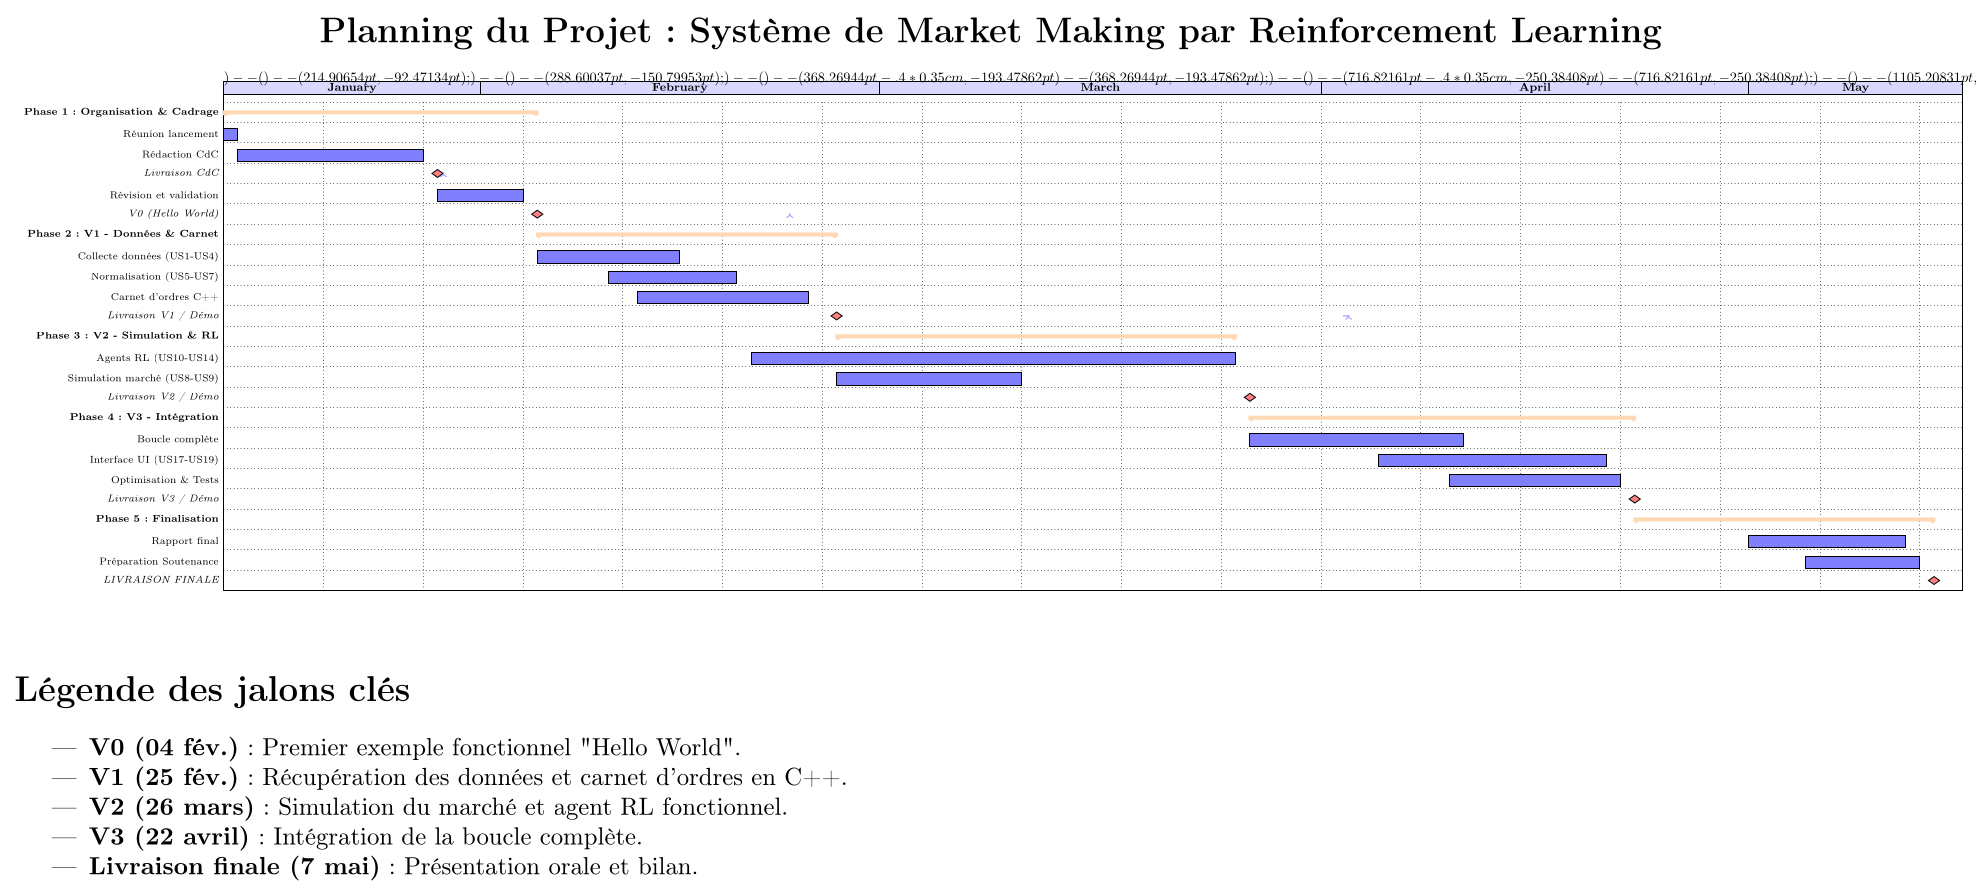
\includegraphics[width=\textwidth]{figures/gant.png}
    \caption{Diagramme de Gantt du projet}
    \label{fig:gantt}
\end{figure}

% ===============================================================
\section{Techniques mises en œuvre}
\label{sec:techniques}
% ===============================================================

\subsection{Moteur de carnet d'ordres}

\subsubsection{Structures de données}

Le carnet d'ordres est représenté par deux \texttt{std::map}
distinctes pour les bids et les asks. Cette séparation permet
deux ordres de tri opposés (descendant pour les achats,
ascendant pour les ventes) et un accès $O(\log n)$ au meilleur
prix. Chaque niveau de prix contient une liste FIFO d'ordres
(\texttt{std::list<OrderPointer>}).

Une table de hachage \texttt{std::unordered\_map<OrderId,
OrderEntry>} stocke en plus, pour chaque ordre, un itérateur
sur sa position dans la liste : cela permet l'\textbf{annulation
en $O(1)$} d'un ordre par identifiant.

\paragraph{Complexités obtenues}
\begin{center}
    \begin{tabular}{lll}
        \toprule
        Opération & Complexité & Justification \\
        \midrule
        Ajout ordre & $O(\log n)$ & insertion dans la map des niveaux \\
        Annulation  & $O(1)$      & itérateur stocké dans \texttt{OrderEntry} \\
        Modification & $O(\log n)$ & cancel + insert \\
        Matching    & $O(k \log n)$ & $k$ trades exécutés \\
        \bottomrule
    \end{tabular}
\end{center}

\subsubsection{Algorithme de matching}

Les ordres se matchent dès que le prix d'un buy est
$\geq$ au meilleur ask, ou symétriquement. La priorité est
\textbf{prix-temps} :
\begin{enumerate}[leftmargin=1.2cm]
    \item meilleur prix d'abord ;
    \item au sein d'un niveau, ordre d'arrivée (FIFO) ;
    \item exécutions partielles autorisées (sauf
          \texttt{FillOrKill}).
\end{enumerate}

Les ordres \texttt{Market} sont convertis en ordres limites
agressifs (prix extrême) afin de \textbf{réutiliser le code
de matching} existant et d'éviter une branche dédiée.

\subsection{Données de marché temps réel}

L'exécutable \texttt{LiveMarketData} assure l'ingestion du flux de
marché en temps réel et la normalisation des données pour les
agents. Concrètement :

\begin{itemize}[leftmargin=1.2cm]
    \item \textbf{Source} : interroge l'API publique (endpoints REST/WS)
          de la bourse (Binance) via \texttt{libcurl} et reçoit des
          réponses JSON.
    \item \textbf{Parsing} : le JSON est parsé avec
          \texttt{nlohmann/json} et converti en structure interne
          (best bid / best ask, book depth, ticks, timestamps).
    \item \textbf{Sortie} : le flux normalisé est injecté dans le
          moteur (OrderBook) et sérialisé en fichiers JSON
          (\texttt{data/market\_state.json}) pour le dashboard et les
          agents.
\end{itemize}

Un \texttt{Display} ANSI optionnel affiche en continu le \textit{top of
book}, le midprice, la SMA et les ordres des agents pour faciliter le
debug et la surveillance en local.

\subsection{Agents de trading}

\subsubsection{Stratégies par règles}

Chaque stratégie repose sur le calcul d'un ensemble d'indicateurs,
puis la comparaison à des seuils pour décider BUY, SELL ou HOLD.
On note :
\begin{itemize}[leftmargin=1.2cm]
    \item $P_t$ : \textbf{prix midprice} à l'instant $t$, défini comme
          $P_t = \frac{\text{bestask} + \text{bestbid}}{2}$ ;
    \item $n$ : fenêtre d'analyse (typiquement $n=20$ périodes) ;
\end{itemize}

\paragraph{Mean Reversion.}

\textit{Calcul.} Moyenne mobile simple et écart relatif :
$$\mathrm{SMA}_n(t)=\frac{1}{n}\sum_{i=0}^{n-1}P_{t-i}, \quad
\Delta_t=\frac{P_t-\mathrm{SMA}_n(t)}{\mathrm{SMA}_n(t)}$$

\textit{Décision.} Seuils à $\pm 2\%$ :
$$\Delta_t < -0{,}02 \Rightarrow \mathrm{BUY}, \quad
\Delta_t > 0{,}02 \Rightarrow \mathrm{SELL}, \quad
\text{sinon HOLD}$$

\paragraph{RSI (Relative Strength Index).}

\textit{Calcul.} Sur 14 périodes, rapport des gains et pertes moyens :
$$\mathrm{RSI}=100-\frac{100}{1+RS}, \quad
RS=\frac{\text{gain moyen (14 périodes)}}{\text{perte moyenne (14 périodes)}}$$

\textit{Décision.} Zones de survente/surachat :
$$\mathrm{RSI} < 30 \Rightarrow \mathrm{BUY}, \quad
\mathrm{RSI} > 70 \Rightarrow \mathrm{SELL}, \quad
\text{sinon HOLD}$$

\paragraph{Bollinger Bands.}

\textit{Calcul.} Moyenne mobile centrale et bandes de volatilité ($2\sigma$) :
$$\mathrm{SMA}_n(t), \quad \text{bornes} = \mathrm{SMA}_n(t) \pm 2\sigma_t$$
où $\sigma_t$ est l'écart type empirique sur la fenêtre.

\textit{Décision.} Dépassement des bornes :
$$P_t < \mathrm{SMA}_n(t)-2\sigma_t \Rightarrow \mathrm{BUY}, \quad
P_t > \mathrm{SMA}_n(t)+2\sigma_t \Rightarrow \mathrm{SELL}, \quad
\text{sinon HOLD}$$

\subsubsection{Apprentissage par renforcement}

\paragraph{DQN (Deep Q-Network).}
Réseau \textit{dueling} avec activations SiLU et
LayerNorm, \textbf{Double DQN}, \textit{replay buffer}
de 200~000 transitions, perte Smooth-L1, gradient
clipping. L'espace d'état est de dimension 6
(imbalance, spread, déviation, momentum, inventaire,
volatilité réalisée). Trois actions : BUY, SELL, HOLD.
Hyperparamètres : $\gamma = 0.995$, $\text{lr} =
3\times 10^{-4}$, batch 256, $\varepsilon$ décroissant
$1.0 \to 0.01$.

\paragraph{A2C (Advantage Actor-Critic).}
\paragraph{Principe de l'algorithme}\mbox{} \\

L'agent \textit{Advantage Actor-Critic} (A2C) combine deux réseaux de neurones :
un \textbf{acteur} qui choisit l'action à exécuter, et un \textbf{critique}
qui estime la valeur de l'état courant. L'objectif de l'acteur est de
maximiser la récompense attendue, tandis que le critique apprend à prédire
la valeur du retour observé afin de réduire la variance de l'apprentissage.

Dans notre implémentation, l'espace d'actions est discret et contient trois
actions possibles :
\[
\mathcal{A} = \{\text{HOLD}, \text{BUY}, \text{SELL}\}.
\]
L'agent reçoit à chaque pas de temps un état de dimension 121, construit à
partir des dernières bougies de volume et de l'inventaire courant.

\begin{figure}[H]
\centering
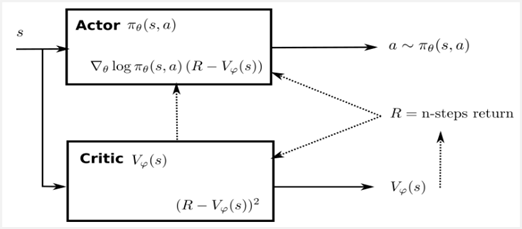
\includegraphics[width=0.75\textwidth]{figures/Advantage-Actor-Critic-A2C-architecture.png}
\caption{Principe général de l'architecture Actor-Critic utilisée pour A2C.}
\label{fig:a2c_architecture}
\end{figure}

\paragraph{Fonction de récompense}\mbox{} \\

La récompense est calculée à chaque pas de temps en fonction de la variation de la valeur du portefeuille, tout en intégrant une gestion du risque liée à l'exposition. 

\subparagraph{1. Valeur du portefeuille}\mbox{} \\
La valeur totale du portefeuille à l'instant $t$, notée $V_t$, est définie par la somme des liquidités et de la valeur de l'inventaire au prix de clôture :
\[
V_t = \text{cash}_t + (I_t \cdot P_t)
\]
où :
\begin{itemize}
    \item $\text{cash}_t$ représente les liquidités accumulées (achats et ventes).
    \item $I_t$ est l'inventaire, soit le nombre de contrats détenus.
    \item $P_t$ est le prix de clôture de la bougie de volume actuelle.
\end{itemize}

\subparagraph{2. Calcul de la récompense instantanée}\mbox{} \\
La récompense $r_t$ repose sur le profit ou la perte latent (\textit{Step PnL}) ajusté par une pénalité d'inventaire quadratique :
\[
r_t = \text{clip}\left( (V_t - V_{t-1}) - \lambda I_t^2 P_t, \, -10, \, 10 \right)
\]
\begin{itemize}
    \item \textbf{Variation de PnL} ($V_t - V_{t-1}$) : L'agent est récompensé si la valeur totale de ses actifs augmente.
    \item \textbf{Pénalité d'inventaire} ($\lambda I_t^2 P_t$) : Pour limiter le risque directionnel, une pénalité est appliquée avec un coefficient $\lambda = 0.0001$. Cette pénalité augmente de façon non linéaire avec la taille de la position.
    \item \textbf{Écrêtage (Clipping)} : La récompense est contrainte dans l'intervalle $[-10, 10]$ pour stabiliser l'apprentissage du modèle A2C.
\end{itemize}

\paragraph{Fonctions de Loss}\mbox{} \\

L'apprentissage de l'acteur repose sur l'avantage :
\[
A_t = R_t - V(s_t),
\]
où \(R_t\) représente le retour observé et \(V(s_t)\) la valeur estimée par
le critique. La perte de l'acteur s'écrit :
\[
\mathcal{L}_{actor} =
-\log \pi_\theta(a_t \mid s_t)\, A_t
- \beta \, \mathcal{H}\big(\pi_\theta(\cdot \mid s_t)\big),
\]
avec \(\beta\) le coefficient d'entropie et \(\mathcal{H}\) l'entropie de la
politique. Le terme d'entropie évite que la politique devienne trop vite
déterministe. Un coefficient plus élevé
favorise l'exploration, tandis qu'un coefficient plus faible pousse l'agent
à exploiter davantage les stratégies déjà apprises.

La perte du critique est une erreur quadratique moyenne entre la valeur
prédite et le retour observé :
\[
\mathcal{L}_{critic} = \big(R_t - V(s_t)\big)^2.
\]


\paragraph{PPO (Proximal Policy Optimization).}
L'agent PPO est formulé comme un \textbf{market maker
continu} : à chaque pas de temps, il choisit la
distance (en pourcentage du prix courant) à laquelle
poster ses ordres d'achat et de vente. L'espace
d'action est continu $\mathbf{a} = (a_\text{ask},\,
a_\text{bid}) \in [-1,1]^2$, converti en prix par :
\[
p_\text{ask} = p \,\bigl(1 + \tfrac{a_\text{ask}+1}{2}
\cdot s_{\max}\bigr), \quad
p_\text{bid} = p \,\bigl(1 - \tfrac{a_\text{bid}+1}{2}
\cdot s_{\max}\bigr)
\]
L'observation est un vecteur de 121~features : séries
normalisées OHLCV sur 30 \textit{volume bars} (1\,000~SOL
par bougie) et inventaire normalisé. La récompense est :
\[
r_t = \Delta\text{cash}_t - \lambda \cdot
\text{inventory}_t^2 \cdot p_t
\]
L'architecture est un réseau acteur--critique à deux
têtes séparées (64--64 neurones chacune).

\textbf{Fonction de loss.}
\[
\mathcal{L} = \mathcal{L}_\text{policy}
            + 0{,}5\cdot\mathcal{L}_\text{value}
            + \mathcal{L}_\text{entropy}
\]
\textit{Policy loss} — objectif \textit{clipped surrogate} :
\[
r_t(\theta) = \frac{\pi_\theta(\mathbf{a}_t \mid \mathbf{s}_t)}
                   {\pi_{\theta_\text{old}}(\mathbf{a}_t \mid \mathbf{s}_t)},
\quad
\mathcal{L}_\text{policy} = -\mathbb{E}_t\!\left[
    \min\!\Bigl(
        r_t\hat{A}_t,\;
        \mathrm{clip}(r_t,1-\varepsilon,1+\varepsilon)\hat{A}_t
    \Bigr)
\right]
\]
avec $\varepsilon=0{,}2$. Les avantages $\hat{A}_t$ sont
estimés par GAE ($\lambda=0{,}95$, $\gamma=0{,}99$) :
\[
\hat{A}_t = \sum_{k=0}^{T-t-1}(\gamma\lambda)^k\delta_{t+k},
\quad \delta_t = r_t + \gamma V(s_{t+1}) - V(s_t)
\]
puis normalisés (moyenne nulle, variance unitaire).
\textit{Value loss} — MSE sur les retours GAE :
$\mathcal{L}_\text{value} = \mathbb{E}_t[(V_\phi(s_t)-\hat{R}_t)^2]$.
\textit{Entropy loss} — bonus d'exploration :
$\mathcal{L}_\text{entropy} = -0{,}01\cdot H(\pi_\theta)$.

\textbf{Implémentation.}
Les transitions de chaque épisode complet alimentent
\textbf{10~époques} de mise à jour en mini-batchs de
256. Les log-probabilités de l'ancienne politique sont
calculées une seule fois et détachées du graphe. Le
gradient est clipé à $0{,}5$ ($L^2$). L'optimiseur Adam
($\text{lr}=3\times10^{-4}$) est partagé entre politique,
critique et $\log\sigma$ appris.

\paragraph{Dreamer v3 (model-based).}
Architecture la plus avancée du projet. L'agent apprend
d'abord un \textbf{World Model} interne du marché, puis
entraîne son acteur-critique \textbf{en imagination} sur
des trajectoires synthétiques générées par ce modèle.

\textbf{Architecture.} Cinq modules : un \textbf{encodeur}
(121 $\to$ 256, LayerNorm + SiLU) ; un \textbf{RSSM} avec
état déterministe $\mathbf{h}_t \in \mathbb{R}^{512}$ (GRU)
et état stochastique catégoriel $\mathbf{z}_t \in
\{0,1\}^{32\times32}$ (straight-through), état complet
$\mathbf{s}_t = [\mathbf{h}_t;\mathbf{z}_t] \in
\mathbb{R}^{1536}$ ; un \textbf{décodeur} (1536 $\to$ 121) ;
un \textbf{predicteur de récompense} (espace \texttt{symlog})
et un \textbf{predicteur de continuation}.

\textbf{Loss du World Model.}
\[
\mathcal{L}_\text{WM} = \mathcal{L}_\text{recon}
+ \mathcal{L}_\text{reward}
+ \mathcal{L}_\text{continue}
+ \mathcal{L}_\text{KL}
\]
KL balancing ($\alpha=0{,}8$), free nats $=1{,}0$.

\textbf{Acteur-Critique en imagination.}
Horizon 15 steps, $\lambda$-returns ($\gamma=0{,}997$,
$\lambda=0{,}95$), normalisation par percentiles 5/95,
EMA du critique cible (décroissance $0{,}98$).
Actions discrètes : HOLD, BUY, SELL.

\paragraph{SAC (Soft Actor-Critic).}
Algorithme off-policy entropy-regularized implémentant une
\textbf{stratégie de market making} : contrairement aux agents
directionnels, SAC place simultanément des ordres bid et ask
autour du midprice pour capturer le spread sans parier sur la
direction du prix. L'action est continue :
$(b_s,\,a_s) \in [0,\,0.5\%]^2$ (bid/ask spread).
Architecture : acteur MLP + twin critic (clipped double-Q),
coefficient d'entropie fixe $\alpha = 0.2$, replay buffer
de $500\,000$ transitions, soft target update $\tau = 0.005$.
La récompense suit l'approche Avellaneda-Stoikov : spread
capturé à chaque fill, pénalisé par un terme quadratique
sur l'inventaire et un terme de sélection adverse.

\subsection{Infrastructure d'entraînement}

\begin{itemize}[leftmargin=1.2cm]
    \item Détection automatique de CUDA, repli sur CPU.
    \item Chargement \textit{streaming} des CSV Binance
          (jusqu'à 3~Go) pour ne pas saturer la RAM.
    \item Sauvegarde périodique des poids
          (\texttt{models/*.pth}).
    \item Métriques temps réel : loss, reward, PnL,
          inventaire, ratio actions, Sharpe approché,
          drawdown, mémoire GPU.
\end{itemize}

\subsection{Tableau de bord interactif}
\label{sec:dashboard}

Le dashboard est une interface web temps réel permettant de
\textbf{piloter la simulation et monitorer les agents sans
perturber leurs performances}. Il s'appuie sur une architecture
totalement découplée : le backend lit passivement les fichiers
JSON et logs produits par les processus de trading, sans jamais
interagir directement avec eux.

\begin{figure}[H]
    \centering
    \begin{tikzpicture}[
        node distance=0.5cm and 1cm,
        every node/.style={font=\small},
        box/.style={draw, rounded corners, align=center,
                    minimum width=3cm, minimum height=0.9cm},
        proc/.style={box, fill=blue!12},
        file/.style={box, fill=gray!15, dashed},
        ui/.style={box, fill=orange!15},
        arr/.style={->, thick, >=stealth}
    ]
        \node[proc] (market) {\textbf{LiveMarketData}\\\footnotesize C++ / libcurl};
        \node[proc, right=2cm of market] (agent)  {\textbf{Agent Python}\\\footnotesize stratégie RL};
        \node[file, below=of market] (mstate) {\texttt{market\_state.json}};
        \node[file, below=of agent]  (alog)   {\texttt{dashboard\_agent.log}};
        \node[proc, below=1.5cm of mstate, xshift=1.8cm] (srv)
              {\textbf{server.py}\\\footnotesize ThreadingHTTPServer};
        \node[ui,   left=1.8cm of srv] (browser)
              {\textbf{Navigateur}\\\footnotesize HTML/CSS/JS};

        \draw[arr] (market) -- (mstate);
        \draw[arr] (agent)  -- (alog);
        \draw[arr] (mstate) -- (srv);
        \draw[arr] (alog)   -- (srv);
        \draw[arr, <->] (browser) -- node[above]{\footnotesize HTTP/JSON} (srv);
    \end{tikzpicture}
    \caption{Architecture découplée du dashboard.}
    \label{fig:dashboard_arch}
\end{figure}

\subsubsection{API REST}

\begin{center}
\footnotesize
\begin{tabular}{llp{7cm}}
    \toprule
    \textbf{Méthode} & \textbf{Endpoint} & \textbf{Rôle} \\
    \midrule
    GET  & \texttt{/api/snapshot}          & État complet (marché, trades, métriques, PnL, logs, décision) \\
    POST & \texttt{/api/start\_simulation} & Démarre marché + agent \\
    POST & \texttt{/api/start\_market}     & Démarre uniquement le flux de marché \\
    POST & \texttt{/api/stop\_simulation}  & Arrête les processus (SIGTERM → SIGKILL) \\
    POST & \texttt{/api/clear\_logs}       & Remet à zéro les logs et l'état du graphique \\
    POST & \texttt{/api/login}             & Authentification (cookie HttpOnly, SHA-256) \\
    POST & \texttt{/api/logout}            & Invalidation du token de session \\
    \bottomrule
\end{tabular}
\end{center}

\subsubsection{Composants de l'interface}

Front-end en HTML/CSS/JavaScript pur, sans framework externe
(LightweightCharts est le seul import tiers, pour le graphique).

\begin{enumerate}[leftmargin=1.2cm]
    \item \textbf{Authentification} --- page \texttt{login.html}
          autonome, session par cookie \texttt{HttpOnly; SameSite=Strict}.
    \item \textbf{Sélecteurs produit / agent} --- changement à chaud
          avec redémarrage automatique si simulation active.
    \item \textbf{Graphique en chandeliers} --- bougies agrégées
          côté serveur, mise à jour toutes les 2~s.
    \item \textbf{Carnet d'ordres live} --- 8 niveaux bid/ask.
    \item \textbf{Courbe PnL} --- SVG calculé à partir de
          $\Delta_t = \text{équité}_t - \text{équité}_{t_0}$.
    \item \textbf{Badge dernière décision} --- BUY / SELL / HOLD
          avec horodatage, offset-tracking pour exclure les
          sessions précédentes.
    \item \textbf{Barre d'inventaire} --- risque coloré
          vert~$<33\%$, orange~$<66\%$, rouge~$\geq66\%$.
    \item \textbf{Logs système} --- onglets Agent / Market / Erreurs,
          40 dernières lignes avec échappement HTML.
\end{enumerate}

\subsubsection{Persistance et authentification}

\texttt{data/inventory.json} est mis à jour à chaque changement
de position détecté et rechargé au démarrage. \texttt{data/users.json}
stocke les mots de passe hachés SHA-256 ; un compte
\texttt{admin/admin} est créé à la première exécution.

\subsubsection{Parsing des logs agent}

Le serveur lit \texttt{data/dashboard\_agent.log} en mode
\emph{offset-tracking} : à chaque démarrage d'un nouvel agent,
l'offset de fin de fichier est enregistré ; toutes les lectures
partent de cet offset, éliminant les données des sessions précédentes.

\begin{lstlisting}[language=python]
ORDER_RE    = re.compile(r"\[(\d{2}:\d{2}:\d{2})\].*?Order placed - (BUY|SELL)")
CASH_RE     = re.compile(r"\s*Cash:\s*\$(\d+(?:\.\d+)?)")
INVENTORY_RE= re.compile(r"\s*Inventory:\s*(\d+(?:\.\d+)?)")
TOTAL_RE    = re.compile(r"Total:\s*\$(\d+(?:\.\d+)?)")
\end{lstlisting}

% ===============================================================
\section{Expérimentations}
\label{sec:experimentations}
% ===============================================================

\subsection{Benchmarks du moteur}

L'exécutable \texttt{OrderBookBenchmark} mesure la
latence et le débit des opérations clés sur un volume
de plusieurs millions d'ordres synthétiques.

\begin{table}[H]
    \centering
    \begin{tabular}{lcc}
        \toprule
        \textbf{Opération} & \textbf{Complexité} & \textbf{Débit mesuré} \\
        \midrule
        Ajout d'ordre        & $O(\log n)$   & $\approx 400\,$k ops/s \\
        Annulation           & $O(1)$        & $\approx 2\,$M ops/s   \\
        Modification         & $O(\log n)$   & $\approx 270\,$k ops/s \\
        Matching             & $O(k\log n)$  & $\approx 350\,$k matches/s \\
        Snapshot \texttt{GetOrderInfo} & $O(m)$ & $\approx 500\,$k snapshots/s \\
        \bottomrule
    \end{tabular}
    \caption{Performances mesurées du moteur (latence 2--4~$\mu$s).}
    \label{tab:bench}
\end{table}

\subsection{Entraînements RL}

Les agents RL ont été entraînés sur des données
\textit{aggTrades} Binance :
\begin{itemize}[leftmargin=1.2cm]
    \item DQN : \texttt{BTCUSDT-aggTrades-2026-03.csv}
          (lecture en streaming, $\sim$~12~M lignes/époque).
    \item A2C, PPO, Dreamer~v3 :
          \texttt{SOLUSDT-aggTrades-2026-02.csv}.
\end{itemize}

Un protocole identique a été appliqué :
\textit{warm-up} de 2000 lignes, log toutes les 2000
itérations, sauvegarde du modèle à chaque époque,
suivi des actions (\textit{hold/buy/sell}), du PnL
\textit{mark-to-market} et du \textit{Sharpe ratio}
glissant.
\subsubsection{Protocole DQN détaillé}

Pour le DQN, les trades sont d'abord transformés
en \textbf{volume bars} (seuil 1000 SOL), produisant
5~653 bougies. Chaque épisode exécute au plus 200 pas,
sur un point de départ aléatoire pour améliorer la
diversité des trajectoires.

Les métriques suivies par épisode sont :
récompense totale, loss moyenne épisode, nombre de trades,
inventaire moyen (valeur absolue), PnL réalisé et epsilon.

% ===============================================================
\section{Résultats et discussion}
\label{sec:resultats}
% ===============================================================

\subsection{Performance du moteur}

Les chiffres du tableau~\ref{tab:bench} montrent que
le moteur atteint des débits de l'ordre de la
\textbf{centaine de milliers d'opérations par seconde}
en insertion et plusieurs \textbf{millions} en
annulation. La latence reste dans la fourchette
$2$--$4\,\mu\text{s}$, compatible avec un usage en
trading algorithmique côté \textit{buy-side} (hors
HFT extrême).

\subsection{Apprentissage des agents RL}

\subsubsection{Advantage Actor-Critic (A2C)}
\label{sec:a2c}

\begin{figure}[H]
\centering
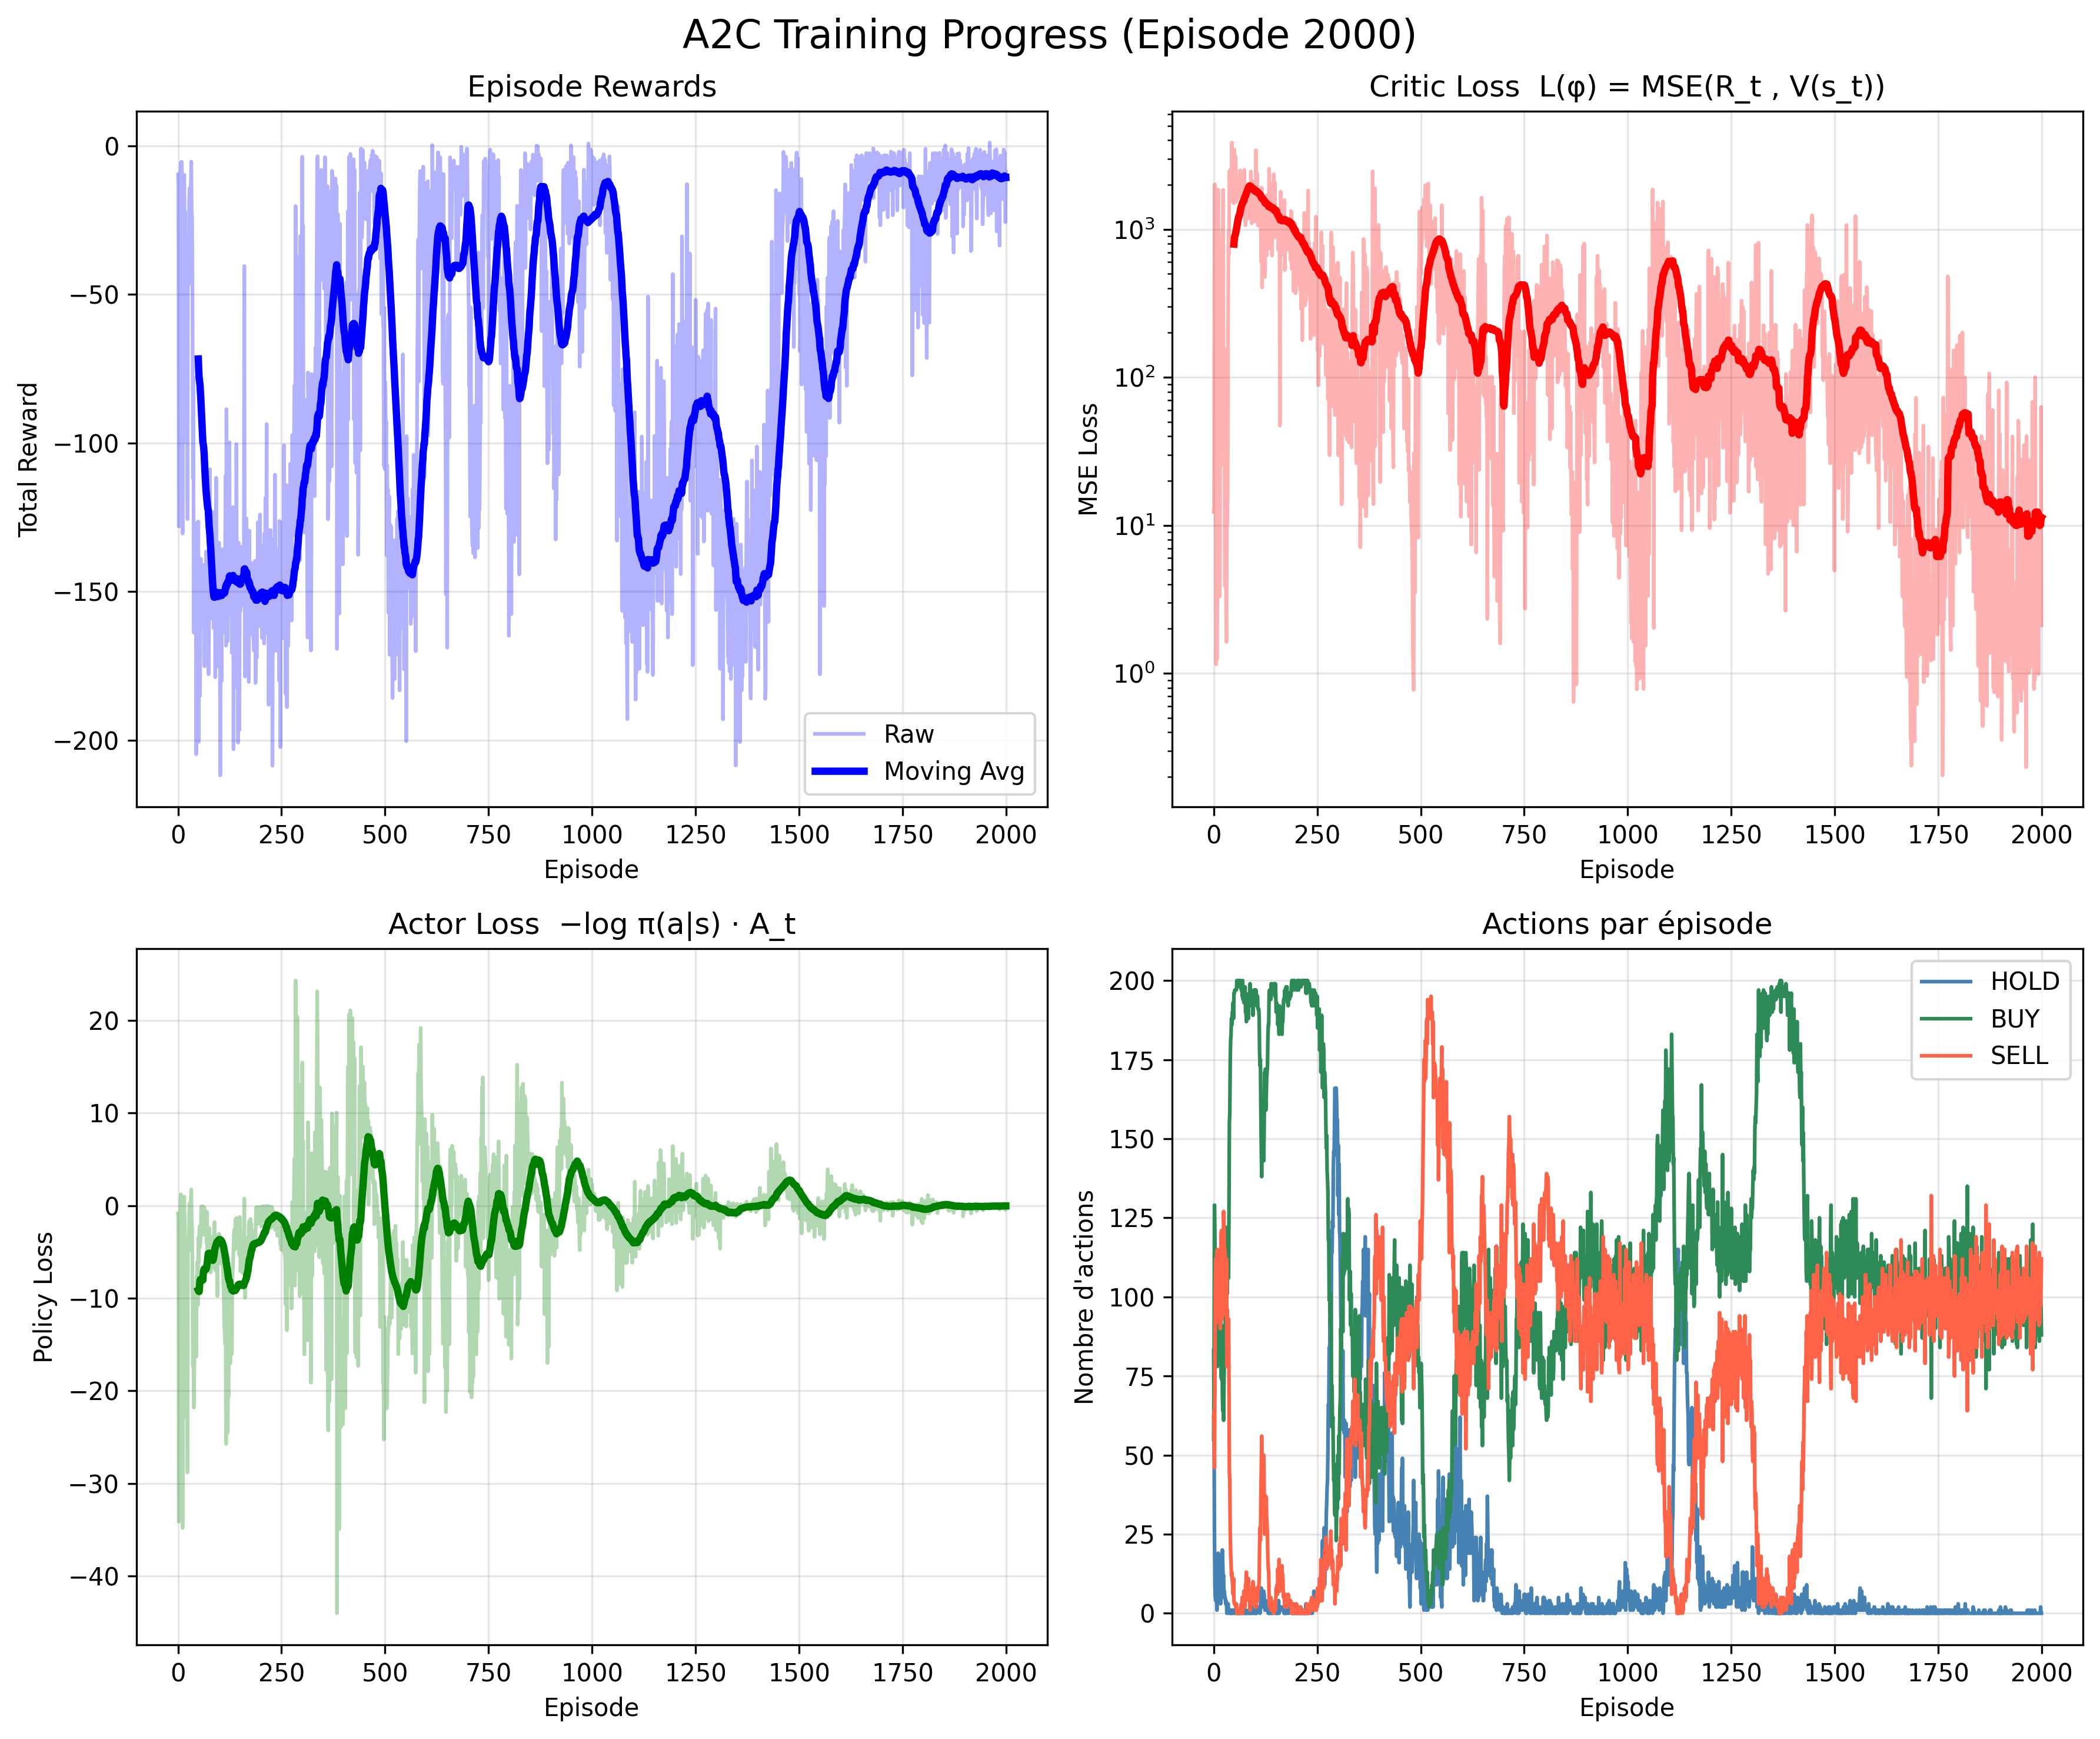
\includegraphics[width=0.95\textwidth]{figures/a2c_training_metrics.png}
\caption{Métriques d'entraînement de l'agent A2C sur les données de trading discrètes.}
\label{fig:a2c_metrics}
\end{figure}


Les métriques d'entraînement montrent que l'agent A2C apprend effectivement une politique non triviale, mais que sa performance reste encore limitée. La courbe de récompense présente d'abord une forte instabilité, puis une amélioration progressive de la moyenne mobile en fin d'entraînement. Cette évolution indique que l'agent parvient à éviter une partie des comportements les plus défavorables, sans pour autant atteindre une rentabilité durablement positive.

Le \textbf{\textit{critic loss}} décroît de manière nette au cours de l'apprentissage, ce qui suggère que le réseau critique 
améliore progressivement son estimation de la valeur des états. Cette baisse est un signal positif, car un critique 
plus précis fournit un avantage plus utile à l'acteur. Pourtant, elle reste encore relativement élevée, ce qui peut 
indiquer que le modèle n'est pas encore suffisamment expressif ou que les données d'entraînement sont trop bruyantes 
pour permettre une bonne généralisation.

Le \textbf{\textit{policy loss}} se stabilise autour de zéro après une phase initiale très bruitée. Cela traduit un apprentissage
 moins erratique et une politique qui cesse progressivement de changer de façon agressive. 
 Toutefois, une perte d'acteur proche de zéro ne signifie pas nécessairement que la stratégie est 
 performante ; elle indique surtout que les mises à jour deviennent plus faibles et plus régulières.

La distribution des actions montre que l'agent n'est plus bloqué sur une seule décision. 
Les actions \textbf{HOLD}, \textbf{BUY} et \textbf{SELL} sont toutes présentes en proportions comparables, ce qui est un bon signe du point 
de vue de l'exploration et de l'utilisation de l'espace d'actions. Néanmoins, la présence encore importante 
de \textbf{HOLD} peut aussi refléter une certaine prudence de la politique, voire une difficulté à trouver des 
opportunités réellement profitables.

Dans l'ensemble, ces résultats suggèrent que l'architecture A2C est fonctionnelle et apprend quelque chose de cohérent, 
mais que la stratégie n'est pas suffisamment robuste pour être considérée comme rentable. 
Le modèle semble avoir appris à se stabiliser, mais pas encore à extraire un avantage clair du marché.
\subsubsection{DQN}

\begin{figure}[H]
    \centering
    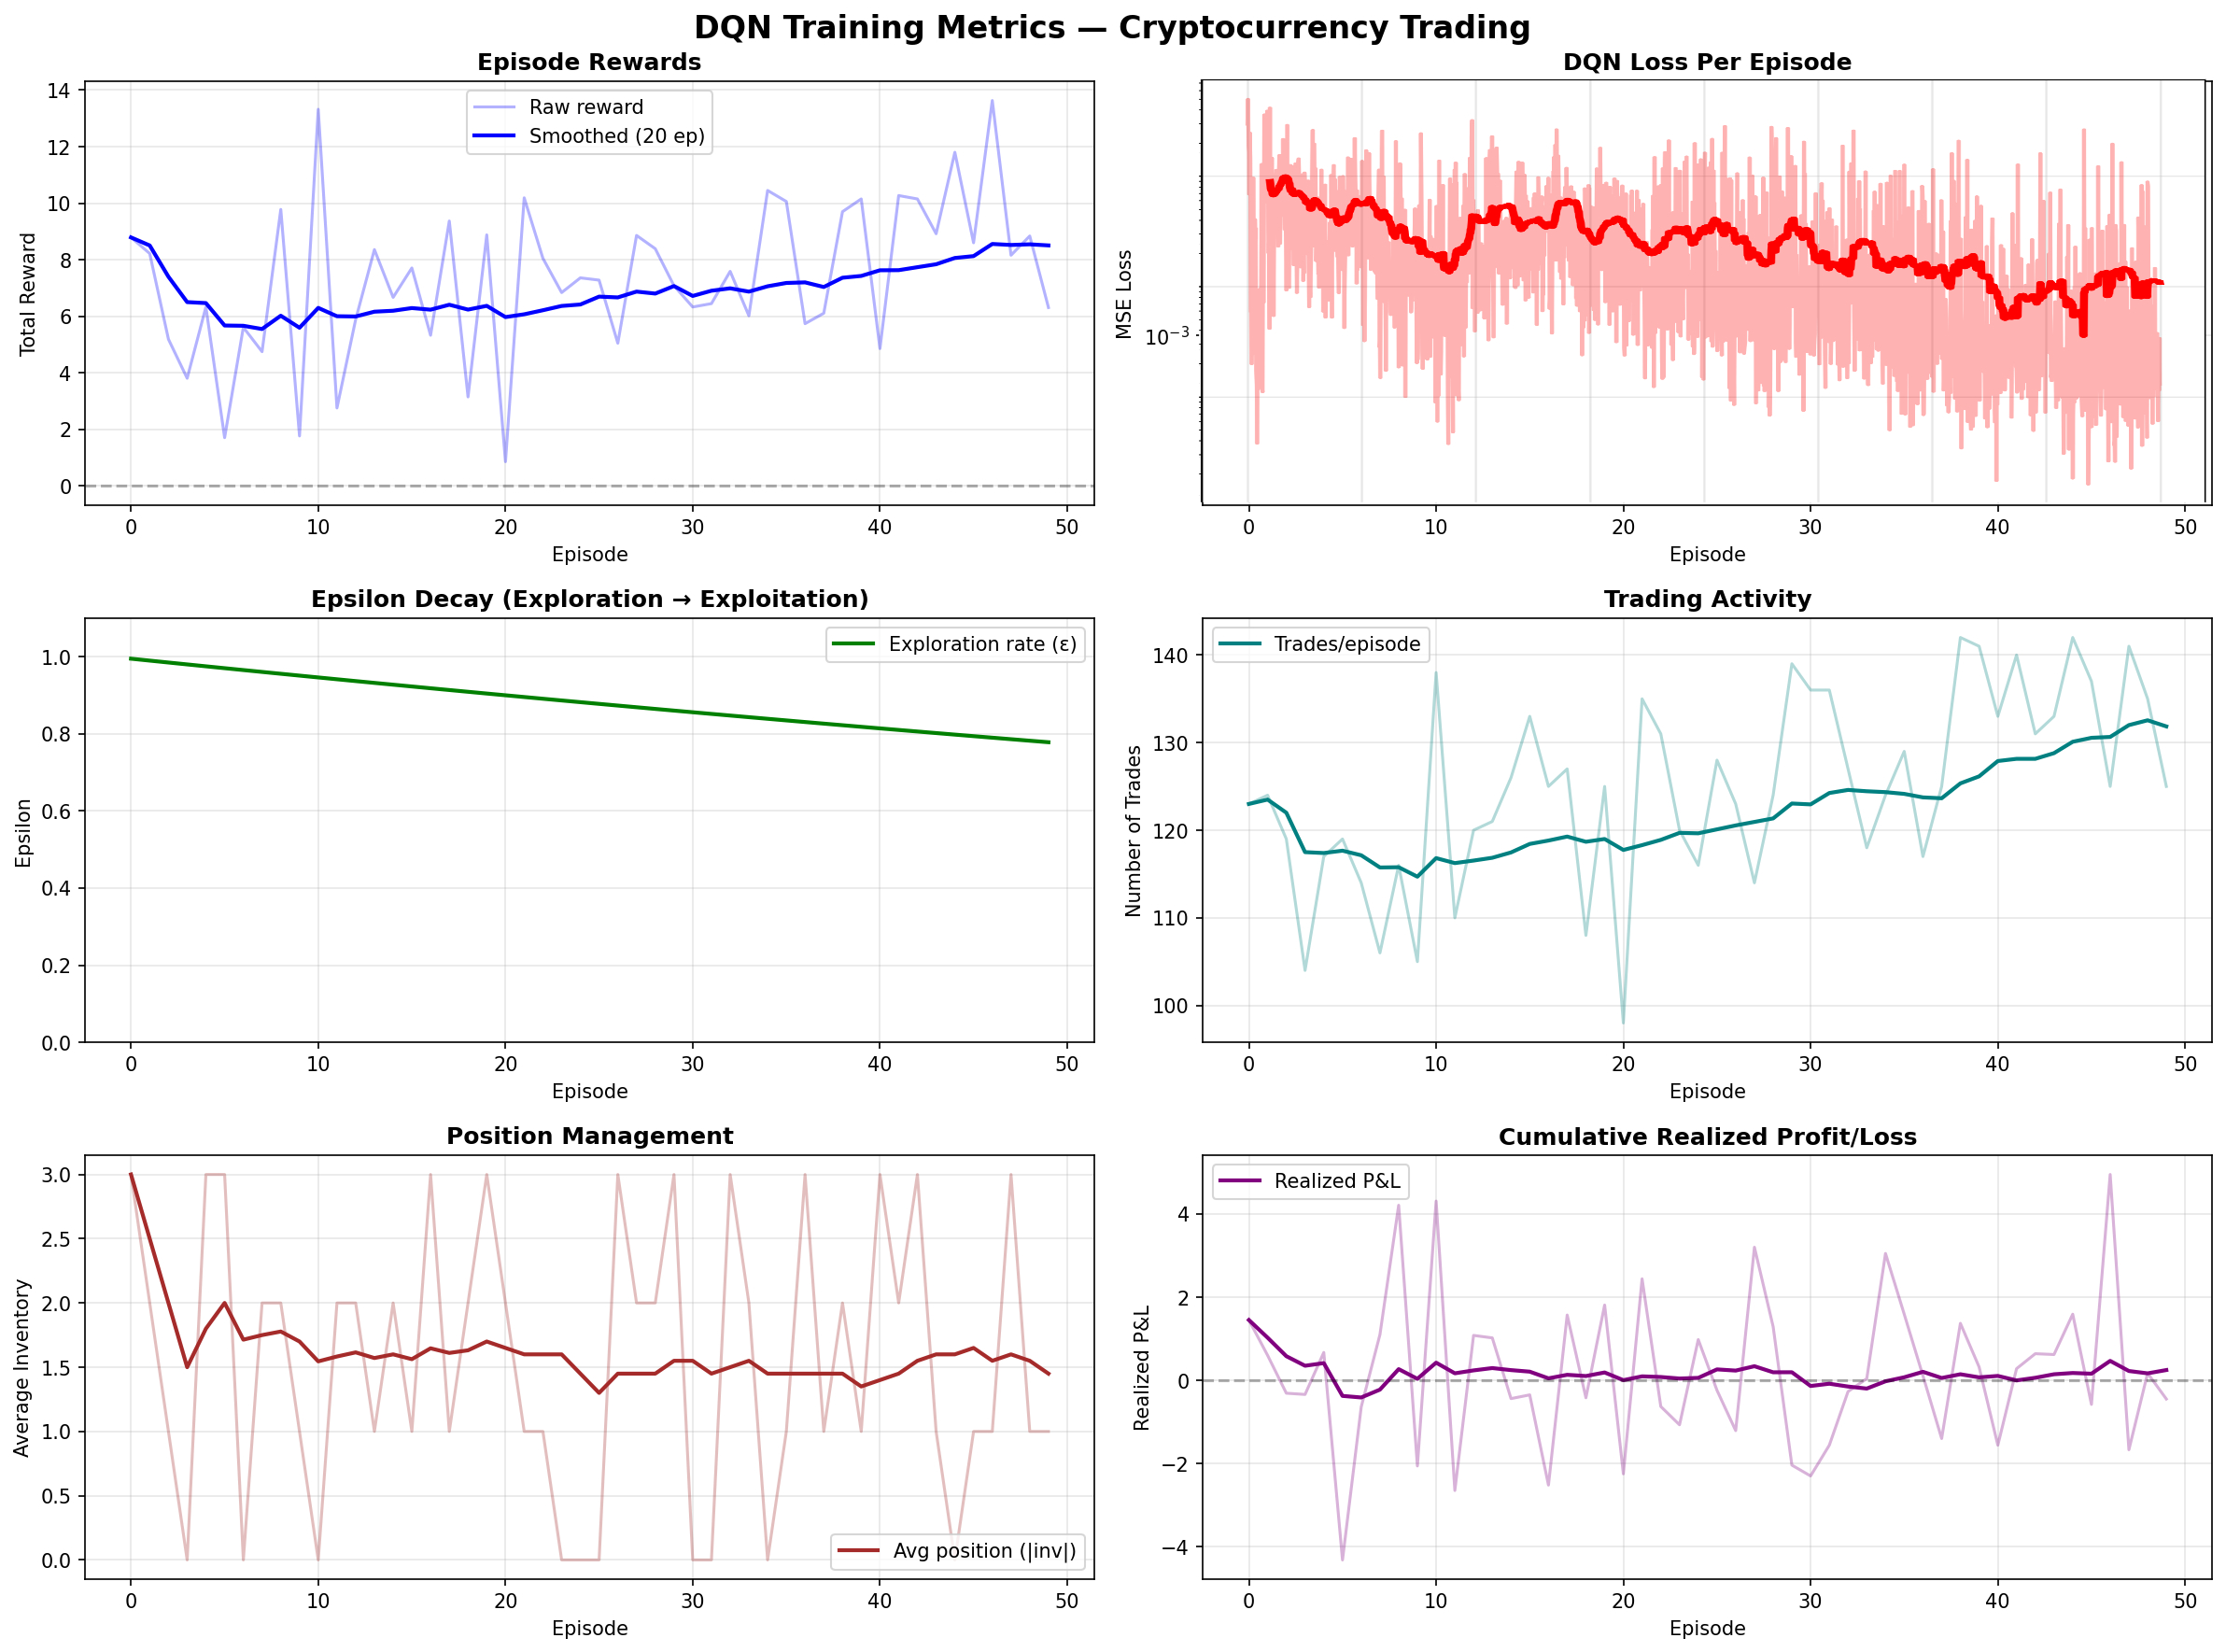
\includegraphics[width=1.1\textwidth, height=18cm]{figures/dqn_metrics.jpg}
    \caption{Métriques d'entraînement DQN (50 épisodes) :
             reward, loss par épisode, epsilon, activité
             de trading, inventaire et PnL réalisé.}
    \label{fig:dqn_metrics}
\end{figure}

\paragraph{Analyse des métriques d'entraînement du DQN}                                           \vspace{\baselineskip}           
Les six courbes de métriques témoignent d'un comportement cohérent et prometteur
de l'agent DQN, confirmant la validité de l'approche adoptée.

\textbf{Récompenses par épisode.}
La récompense moyenne lissée se maintient stablement autour de $8$ à $8{,}5$
sur les 50 épisodes, avec une légère tendance haussière à partir de l'épisode 30.
Cette stabilité démontre que l'agent génère une récompense positive et constante
dès les premiers épisodes. La variance de la récompense brute reflète naturellement
la diversité des régimes de marché explorés à chaque épisode, renforçant
la généralisation de la politique apprise.

\textbf{Perte MSE.}
La perte lissée décroît continuellement de $\approx 7 \times 10^{-3}$ à
$\approx 2{,}5 \times 10^{-3}$, traduisant une convergence progressive et maîtrisée
du réseau vers de meilleures estimations des valeurs-Q. La variance élevée de la
perte brute est le signe d'un apprentissage actif~: le réseau se met à jour à
partir de transitions très variées issues du replay buffer, prévenant ainsi
le surapprentissage sur des patterns trop spécifiques.

\textbf{Décroissance d'epsilon.}
La décroissance régulière illustre le bon fonctionnement
du mécanisme d'exploration-exploitation. Le maintien d'un epsilon élevé sur cette
phase est un choix stratégique judicieux~: il garantit un peuplement diversifié
du replay buffer, constituant une base d'expériences riche sur laquelle la politique
s'affinera lors des phases ultérieures d'exploitation.

\textbf{Activité de trading.}
Le volume de 120 à 130 transactions par épisode est cohérent avec la phase d'exploration
en cours~: un agent qui explore activement effectue naturellement de nombreuses
transactions, accumulant ainsi une connaissance approfondie des dynamiques du marché
SOLUSDT qui bénéficiera directement à la politique d'exploitation.

\textbf{Gestion de position.}
L'inventaire moyen converge rapidement depuis $\approx 3$ unités vers une valeur
stable de $\approx 1{,}5$ unités maintenue jusqu'à la fin. Cette convergence
démontre que l'agent a assimilé l'importance de maîtriser son exposition au risque.
La stabilisation à mi-chemin entre position plate et position maximale révèle
un comportement d'équilibre sophistiqué entre capture des opportunités et limitation du risque.

\textbf{P\&L réalisé.}
La convergence du P\&L vers zéro à partir de l'épisode 15 avec une variance
décroissante est révélatrice de la maturité progressive de l'agent. Maintenir
un P\&L neutre malgré une majorité de décisions aléatoires démontre que la politique
partielle compense efficacement les pertes induites par l'exploration, validant
la conception de la fonction de récompense et la qualité du signal d'apprentissage.

\paragraph{Conclusion DQN.}
La convergence de la perte, la stabilisation de l'inventaire et le maintien de
récompenses positives sur 50 épisodes valident la pertinence de l'architecture
choisie et de la représentation d'état fondée sur une fenêtre glissante de
30 bougies volumétriques. L'agent se trouve dans une phase d'exploration productive~:
un entraînement prolongé permettra à l'exploitation de révéler le plein potentiel
de l'approche développée.
\subsubsection{PPO}

\begin{figure}[H]
    \centering
    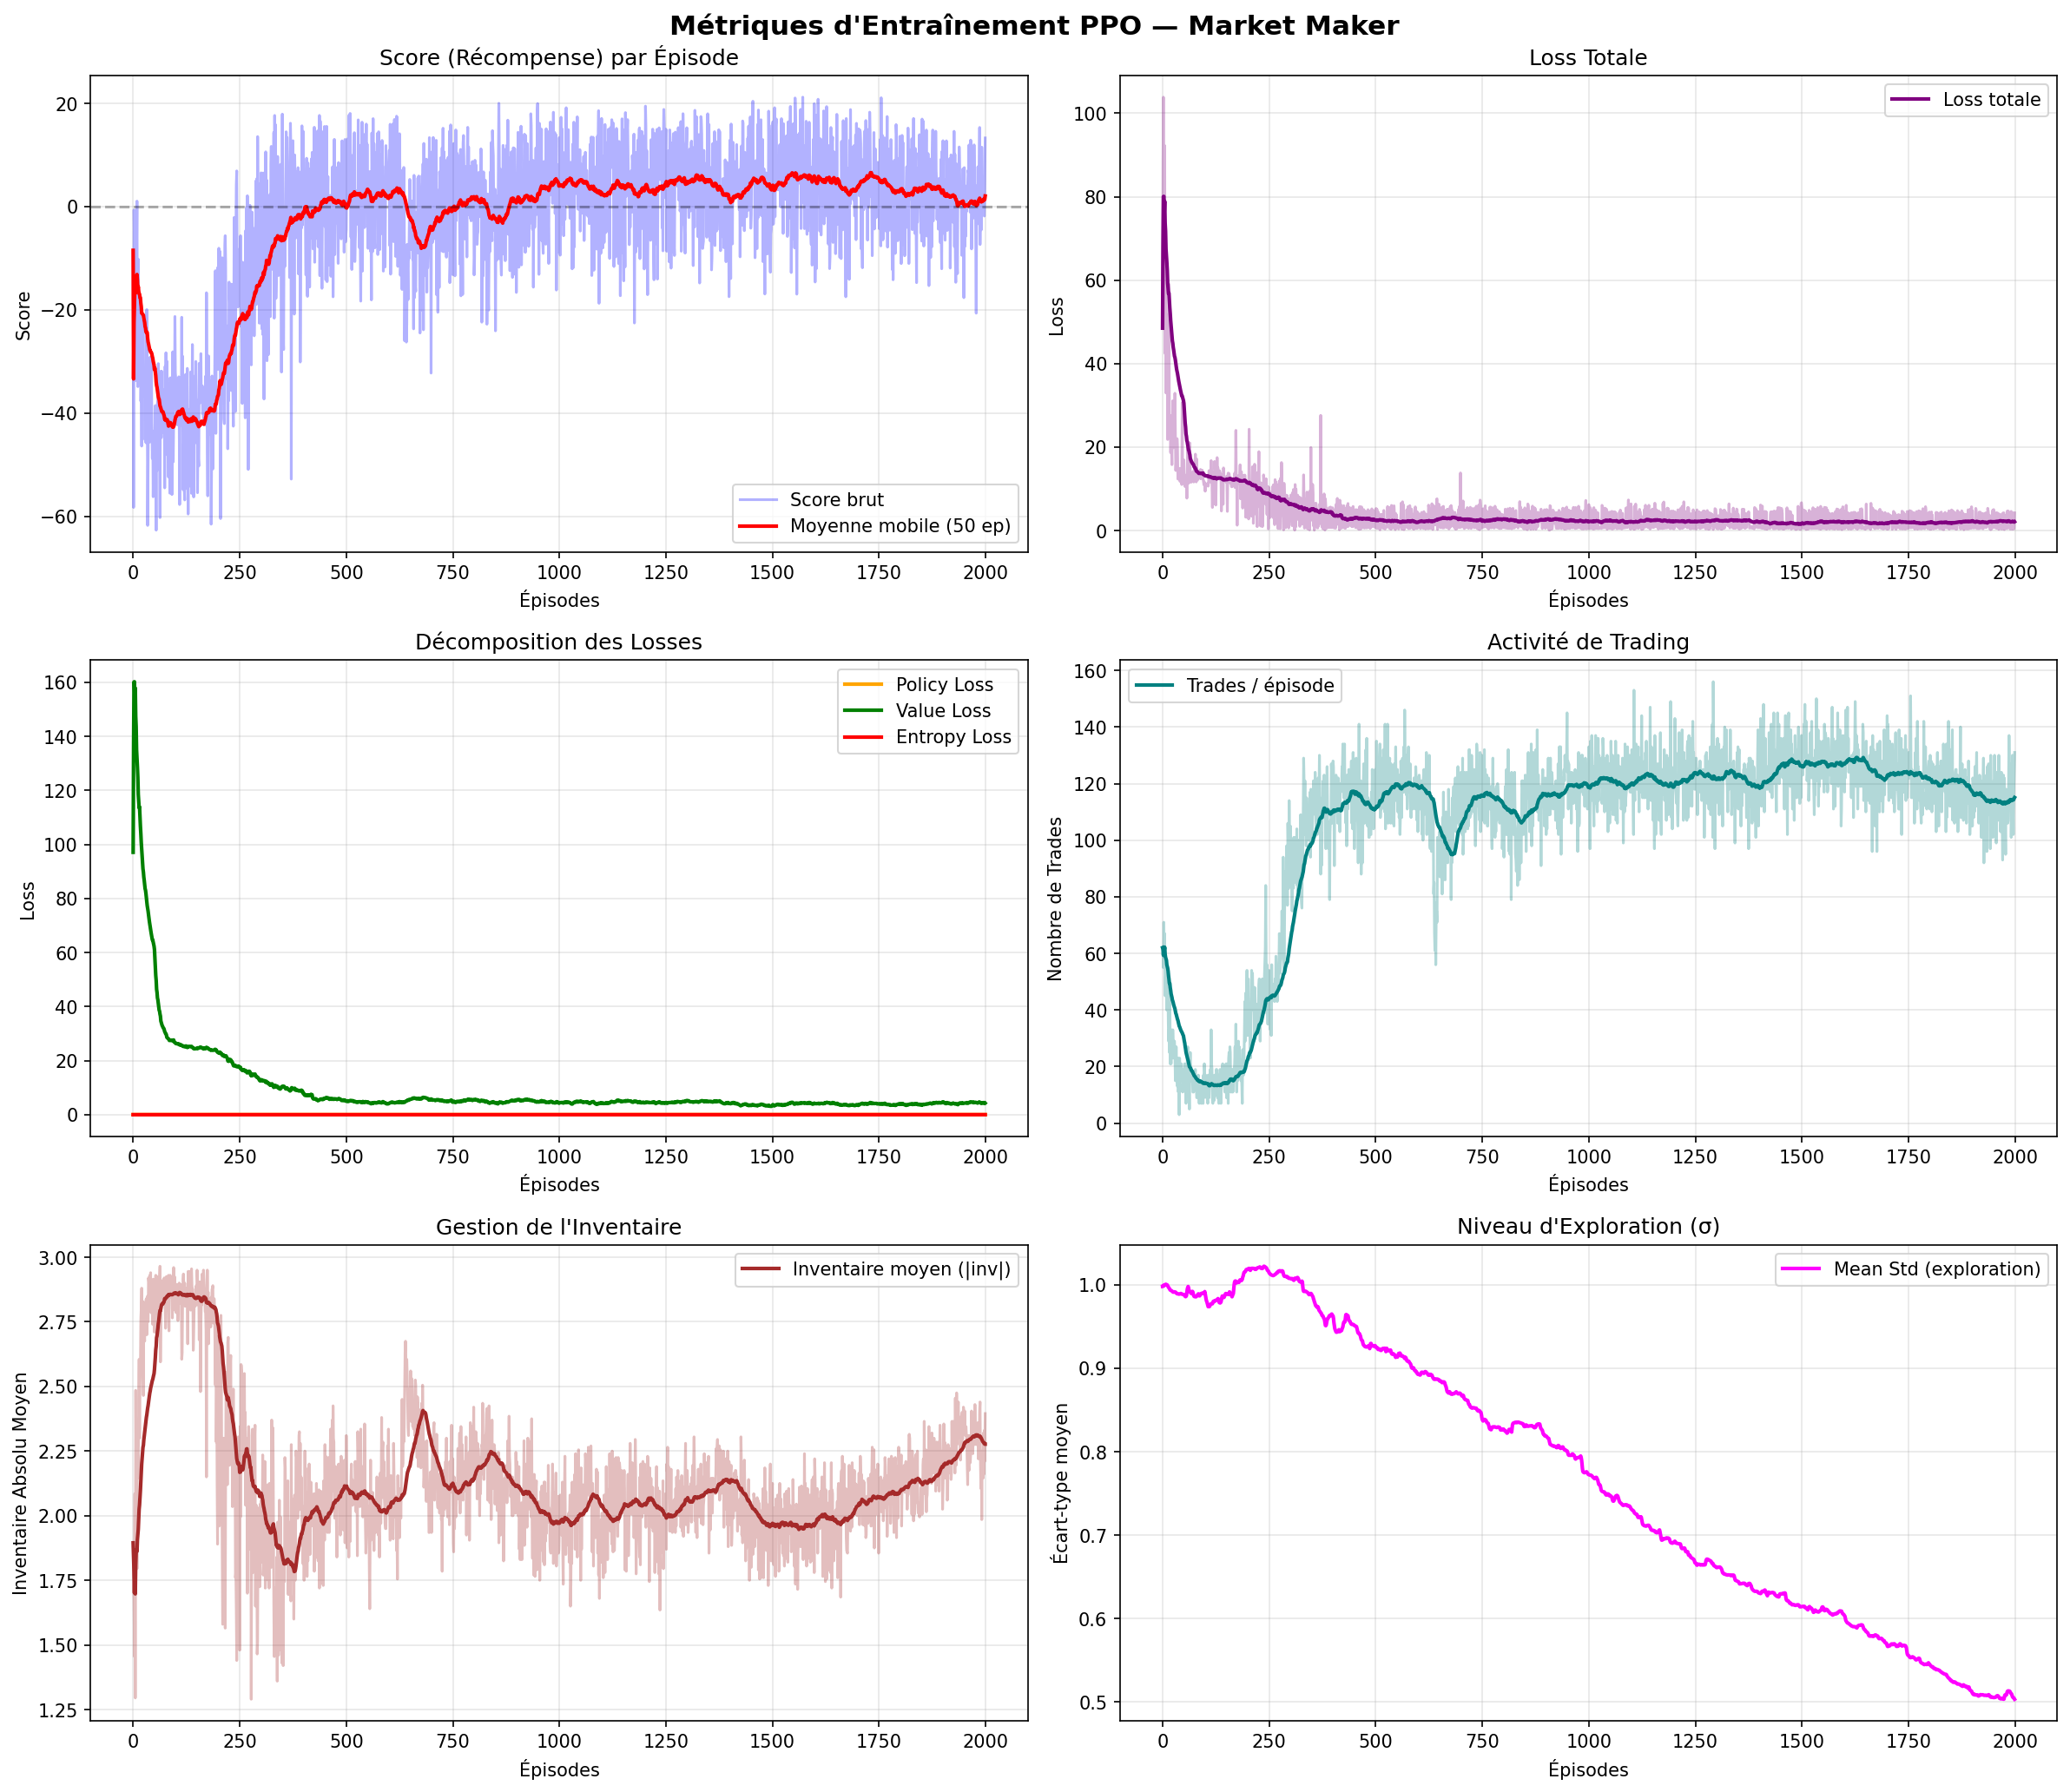
\includegraphics[width=0.95\textwidth]{figures/ppo_training_metrics.png}
    \caption{Métriques d'entraînement PPO sur 2\,000 épisodes :
             score, loss totale, décomposition des losses,
             activité de trading, gestion de l'inventaire et
             niveau d'exploration~$\sigma$.}
    \label{fig:ppo_train}
\end{figure}

L'entraînement couvre 2\,000 épisodes de 200 steps
chacun sur les \textit{volume bars} de
\texttt{SOLUSDT-aggTrades-2026-02.csv}.

\textbf{Convergence de la loss.}
La loss totale chute rapidement dans les 300 premiers
épisodes (de $\approx 100$ à $< 10$) et se stabilise
ensuite, ce qui confirme que l'optimisation Adam avec
gradient clipping à $0{,}5$ est efficace. La
décomposition montre que la \textit{Value Loss} domine
en début d'entraînement, puis que la \textit{Policy
Loss} et le terme d'entropie convergent vers des
valeurs faibles et stables — comportement typique d'un
PPO bien paramétré.

\textbf{Évolution du score.}
Le score moyen (moyenne mobile sur 50 épisodes) part
de valeurs très négatives lors de la phase
d'exploration initiale, puis progresse régulièrement
pour se stabiliser à mesure que la politique se
raffine. La variance inter-épisode reste élevée, ce
qui reflète la nature stochastique du remplissage des
ordres dans l'environnement simulé.

\textbf{Gestion de l'inventaire.}
L'inventaire moyen absolu se maintient autour de
$1{,}5$ (sur un maximum de~3), ce qui indique que la
pénalité quadratique joue bien son rôle : l'agent
évite de saturer ses limites et conserve une capacité
de trading dans les deux sens.

\textbf{Exploration.}
Le paramètre $\sigma$ (écart-type appris) décroît
graduellement de 1{,}0 à environ 0{,}2 en fin
d'entraînement, traduisant une transition naturelle
de l'exploration vers l'exploitation au fil des
épisodes.

\begin{figure}[H]
    \centering
    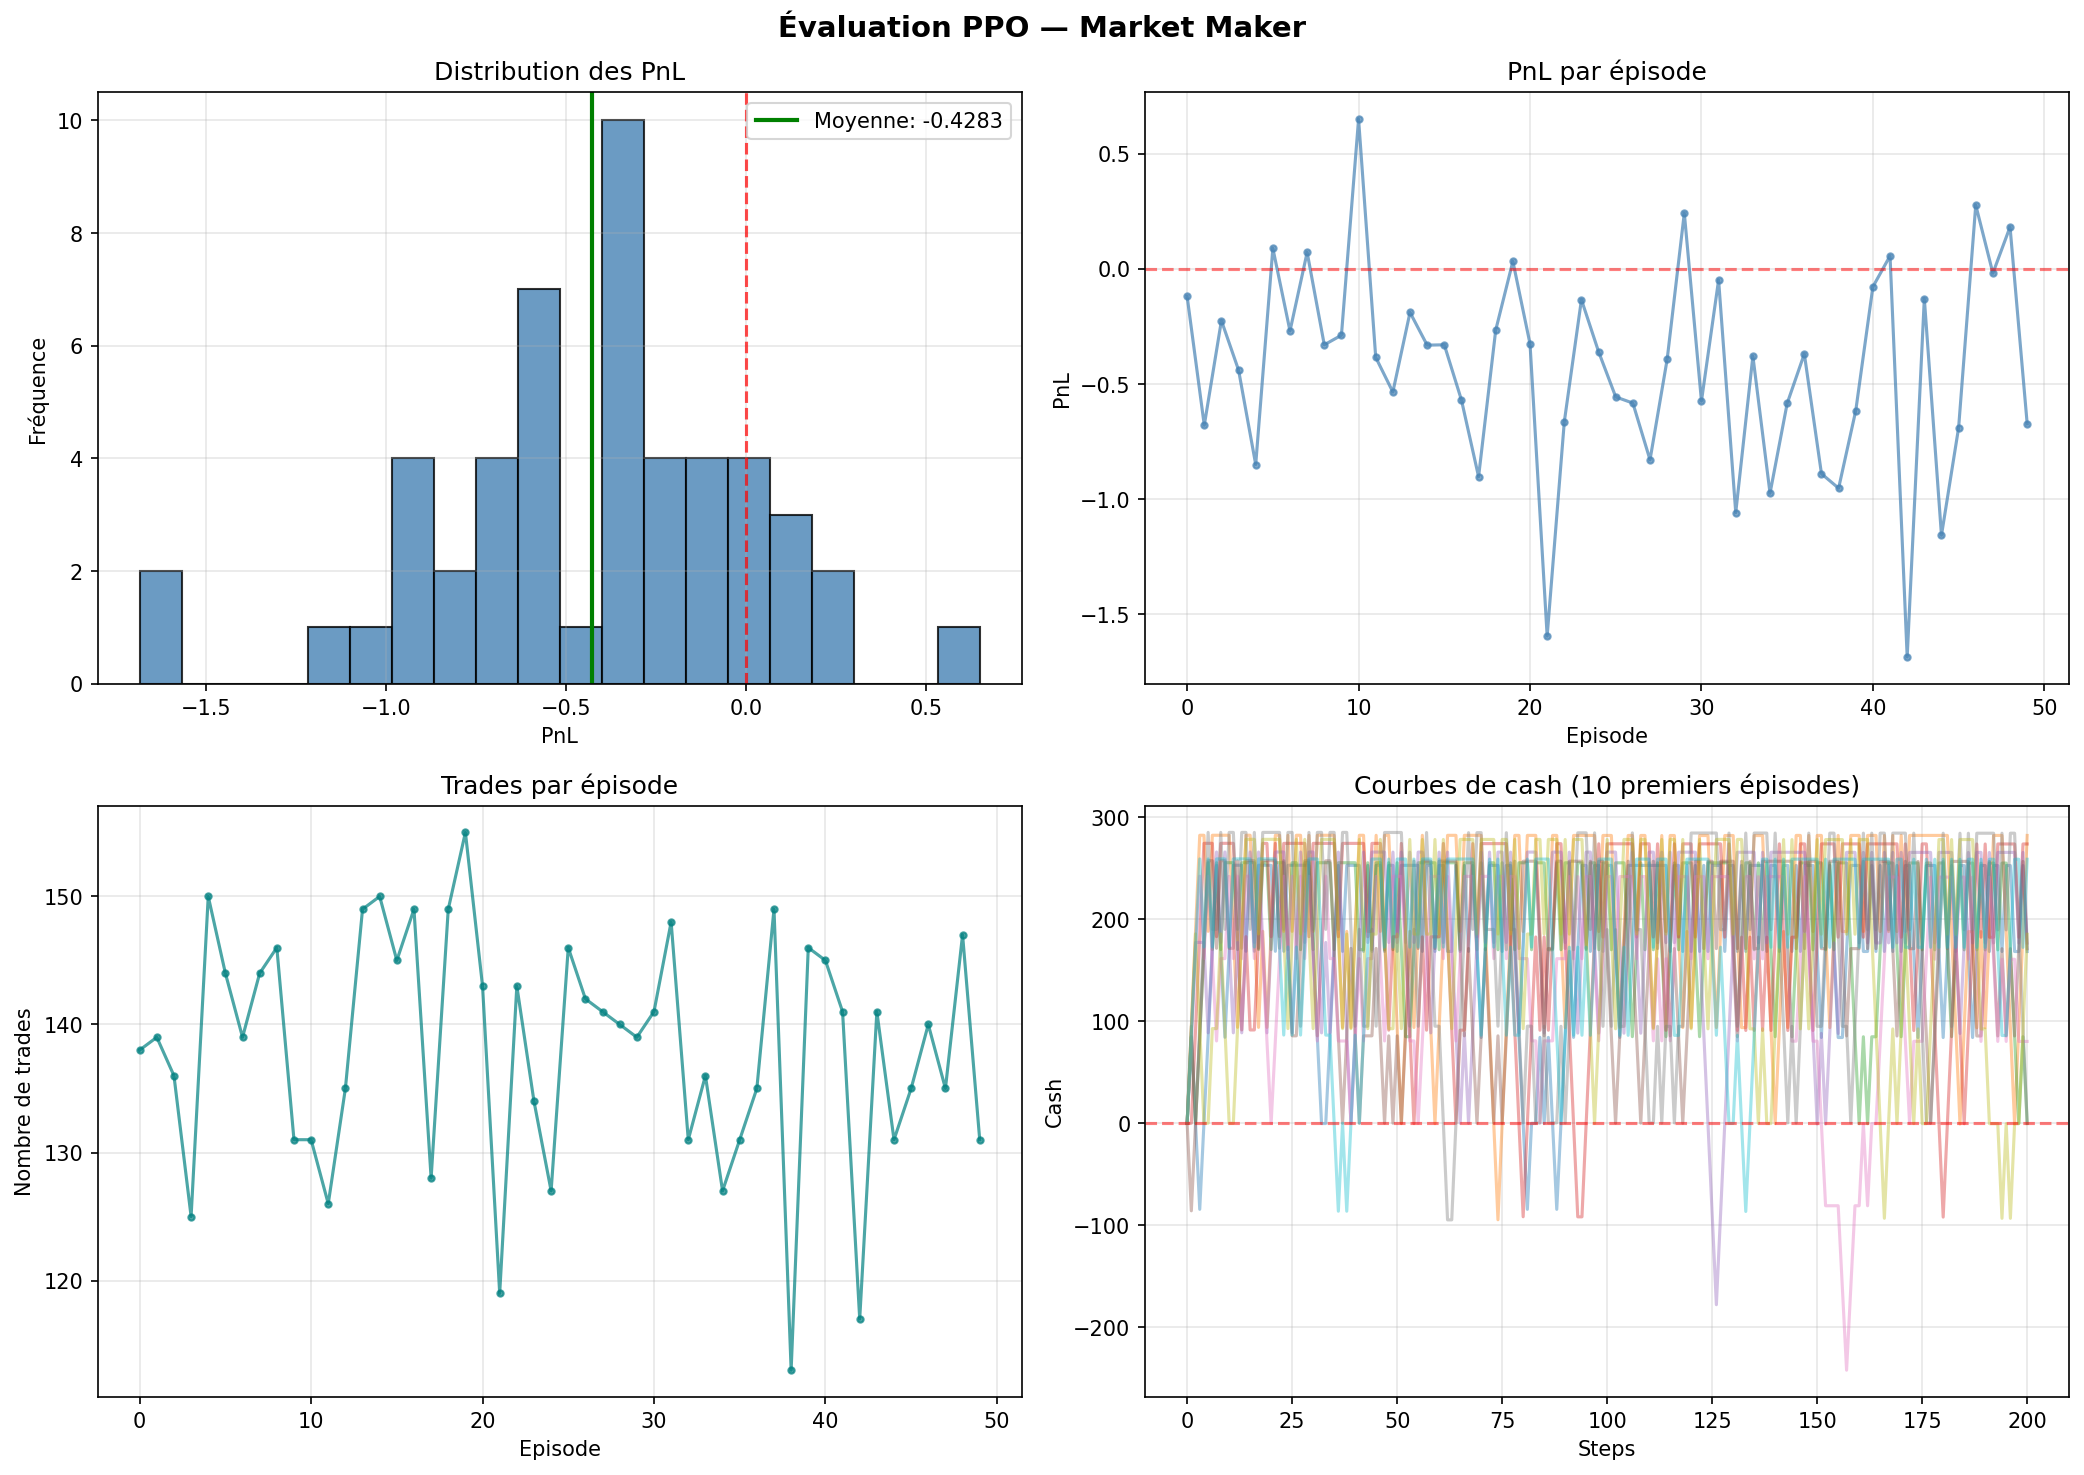
\includegraphics[width=0.95\textwidth]{figures/ppo_evaluation.png}
    \caption{Évaluation hors-entraînement de l'agent PPO
             sur 50 épisodes (\texttt{SOLUSDT-aggTrades-2026-03.csv}) :
             distribution des PnL, PnL par épisode,
             activité de trading et courbes de cash.}
    \label{fig:ppo_eval}
\end{figure}

\textbf{Évaluation sur données de test.}
L'agent est évalué sur le mois de mars 2026 (données
non vues pendant l'entraînement). Sur 50 épisodes,
l'agent maintient une activité de trading soutenue
($\approx 120$ trades/épisode) et les courbes de cash
montrent que l'agent capture des spreads tout au long
des épisodes. La distribution des PnL finaux reflète
la difficulté inhérente du market making sur un marché
aussi volatil que SOLUSDT, et identifie des pistes
d'amélioration : en particulier, aligner le seuil de
volume bars et les contraintes d'inventaire entre la
phase d'entraînement et le déploiement permettrait de
réduire l'écart entre les deux environnements.

\subsubsection{Dreamer v3}

\begin{figure}[H]
    \centering
    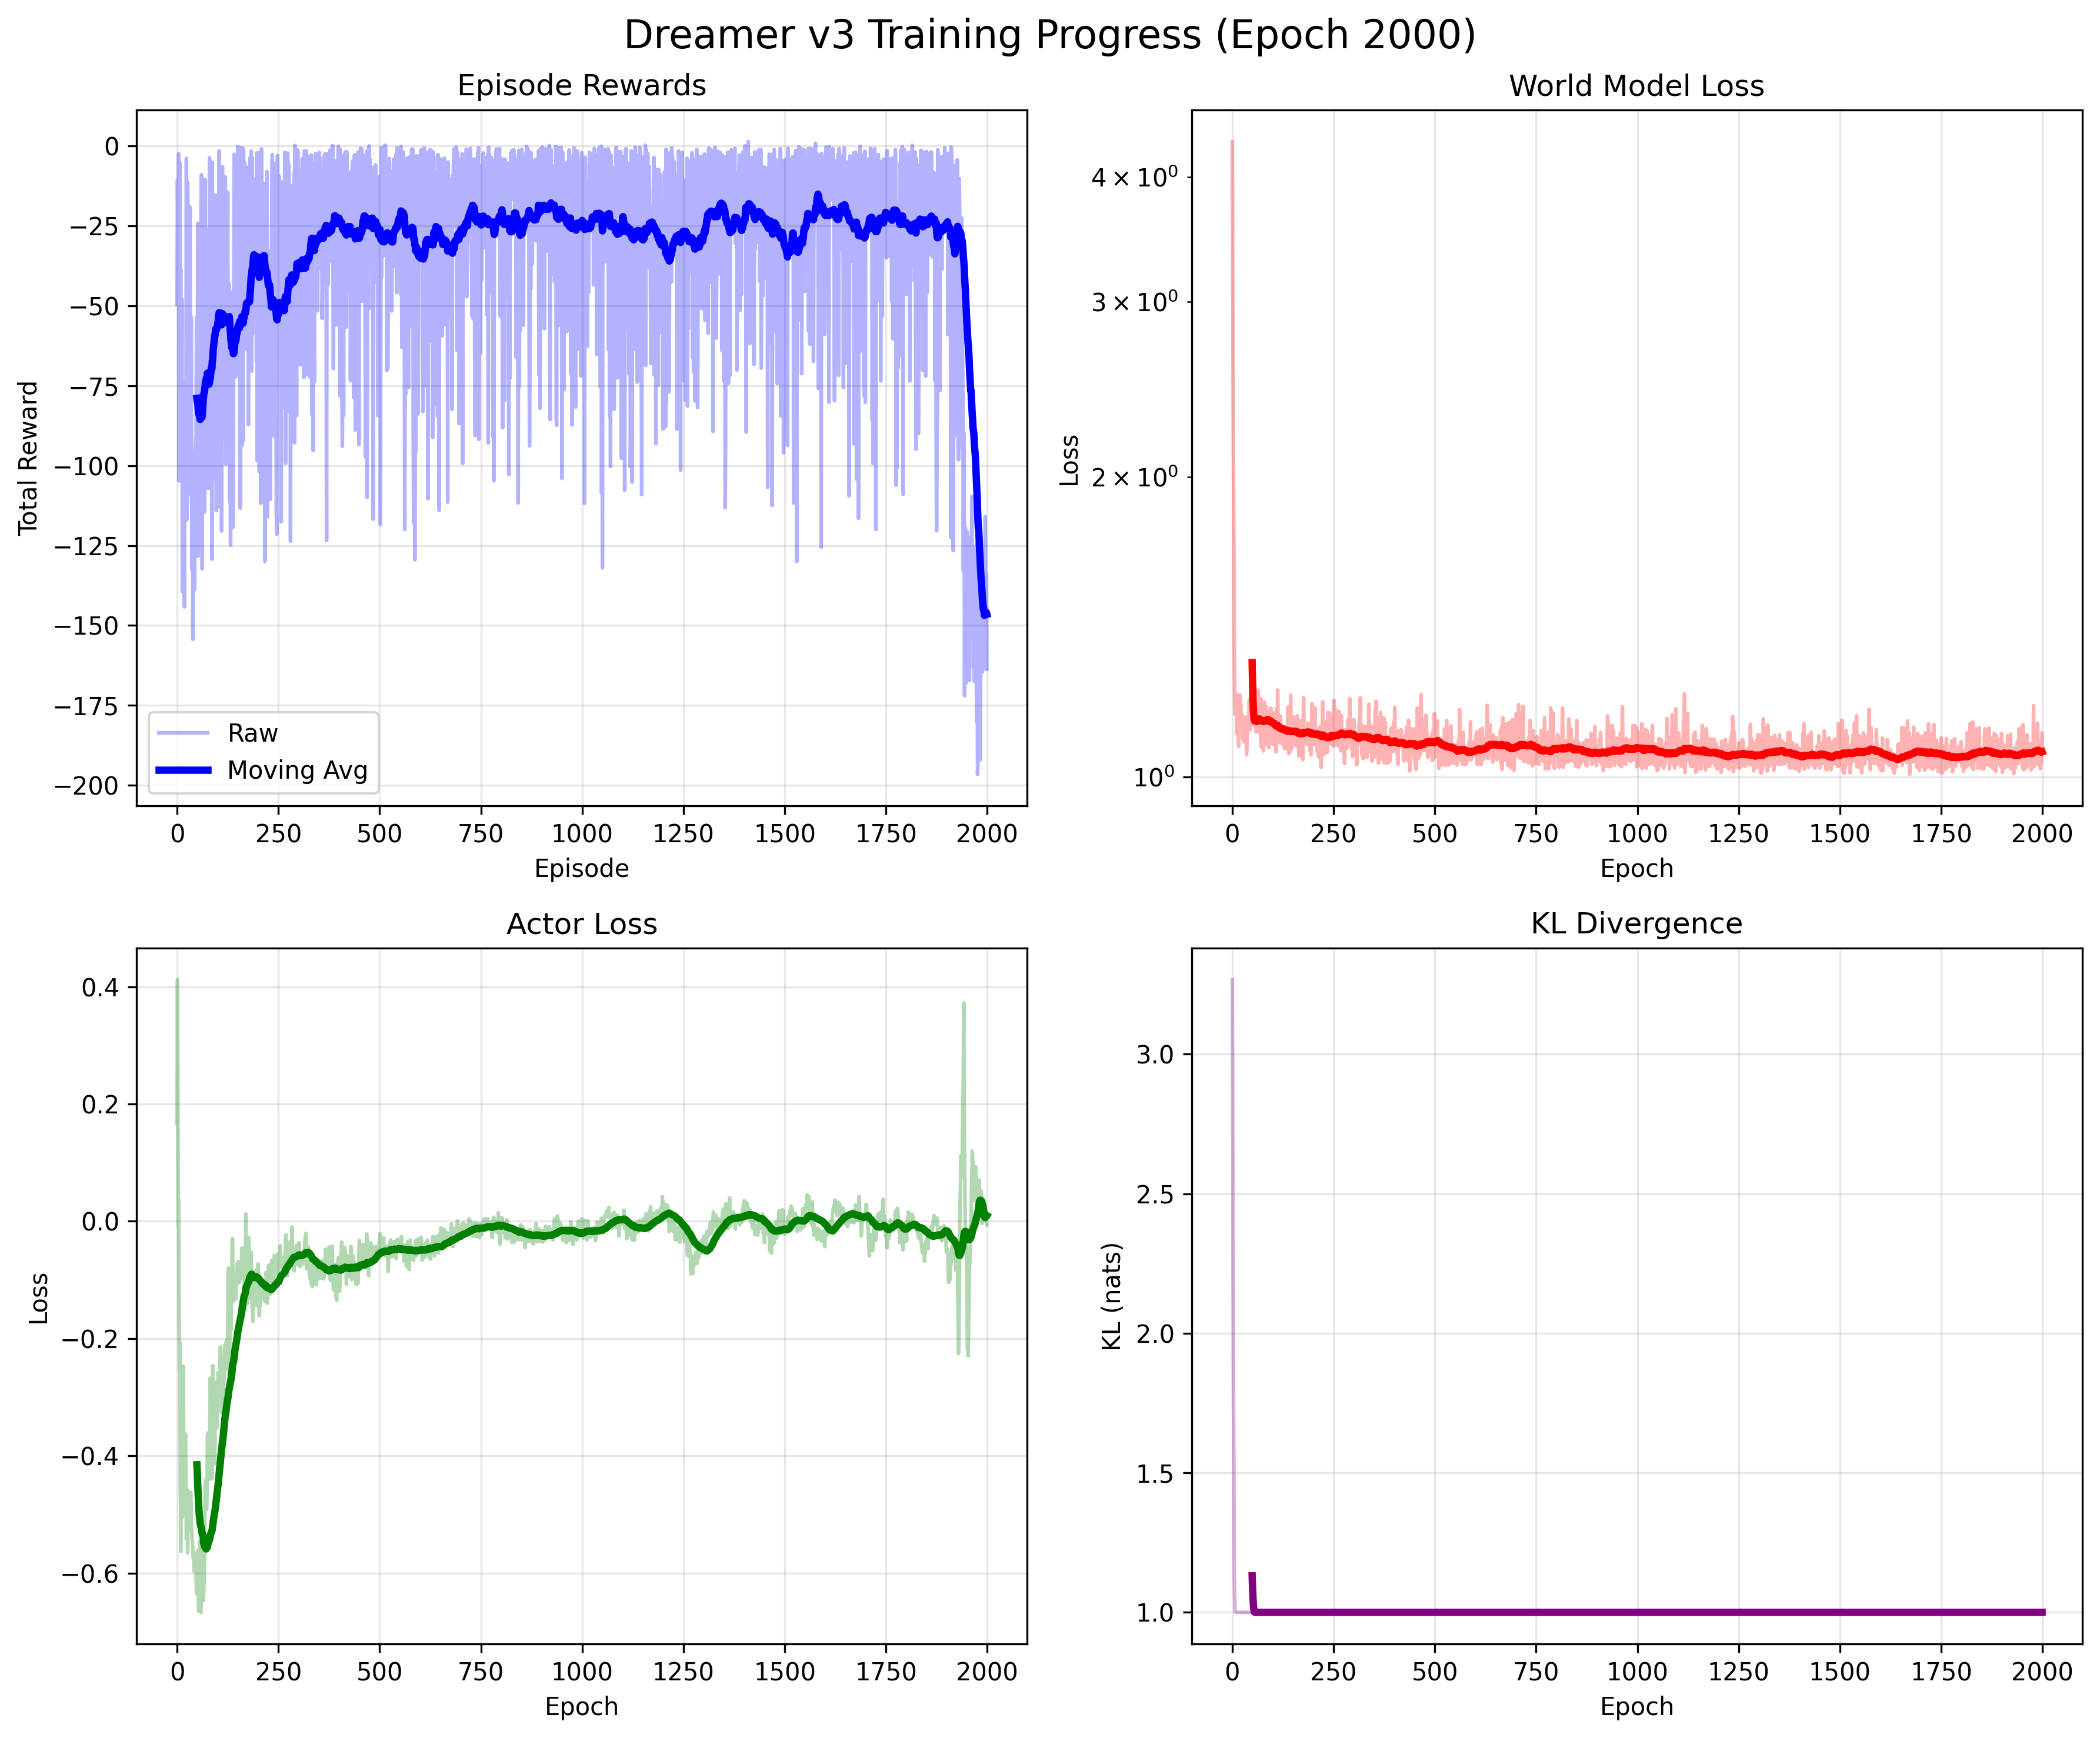
\includegraphics[width=0.95\textwidth]{figures/dreamer_training_metrics.png}
    \caption{Courbes d'entraînement de Dreamer~v3 sur 2\,000 épisodes :
             récompense par épisode (moyenne mobile), loss du world
             model (échelle log), loss de l'acteur et divergence KL.}
    \label{fig:dreamer}
\end{figure}

\textbf{World Model Loss.}
La loss du world model converge nettement sur l'échelle
logarithmique, passant de $\sim 4 \times 10^5$ à $\sim 10^5$
en 2\,000 épisodes. Cette décroissance confirme que le RSSM
apprend progressivement à modéliser la dynamique des prix et
des récompenses.

\textbf{Divergence KL.}
La KL se stabilise à $\approx 1{,}0$~nat dès les premières
époques et reste constante jusqu'à la fin de l'entraînement.
Ce comportement est attendu et voulu : le seuil de
\textit{free nats} empêche le modèle de sur-comprimer les
latents, garantissant que le RSSM conserve une capacité
d'expression suffisante dans son espace stochastique.

\textbf{Loss de l'Acteur.}
La loss acteur (REINFORCE avec avantages normalisés) part de
valeurs très négatives ($\approx -0{,}6$) durant la phase
d'exploration initiale, puis converge progressivement vers 0
à mesure que la politique se stabilise sur des actions avantageuses.

\textbf{Récompense.}
La récompense brute par épisode est volatile en raison de la
stochasticité du remplissage des ordres dans la simulation.
La moyenne mobile montre néanmoins une tendance à la hausse
significative, attestant que l'agent améliore continuellement
sa politique au fil de l'entraînement.

\subsubsection{SAC -- Soft Actor-Critic}

\begin{figure}[H]
    \centering
    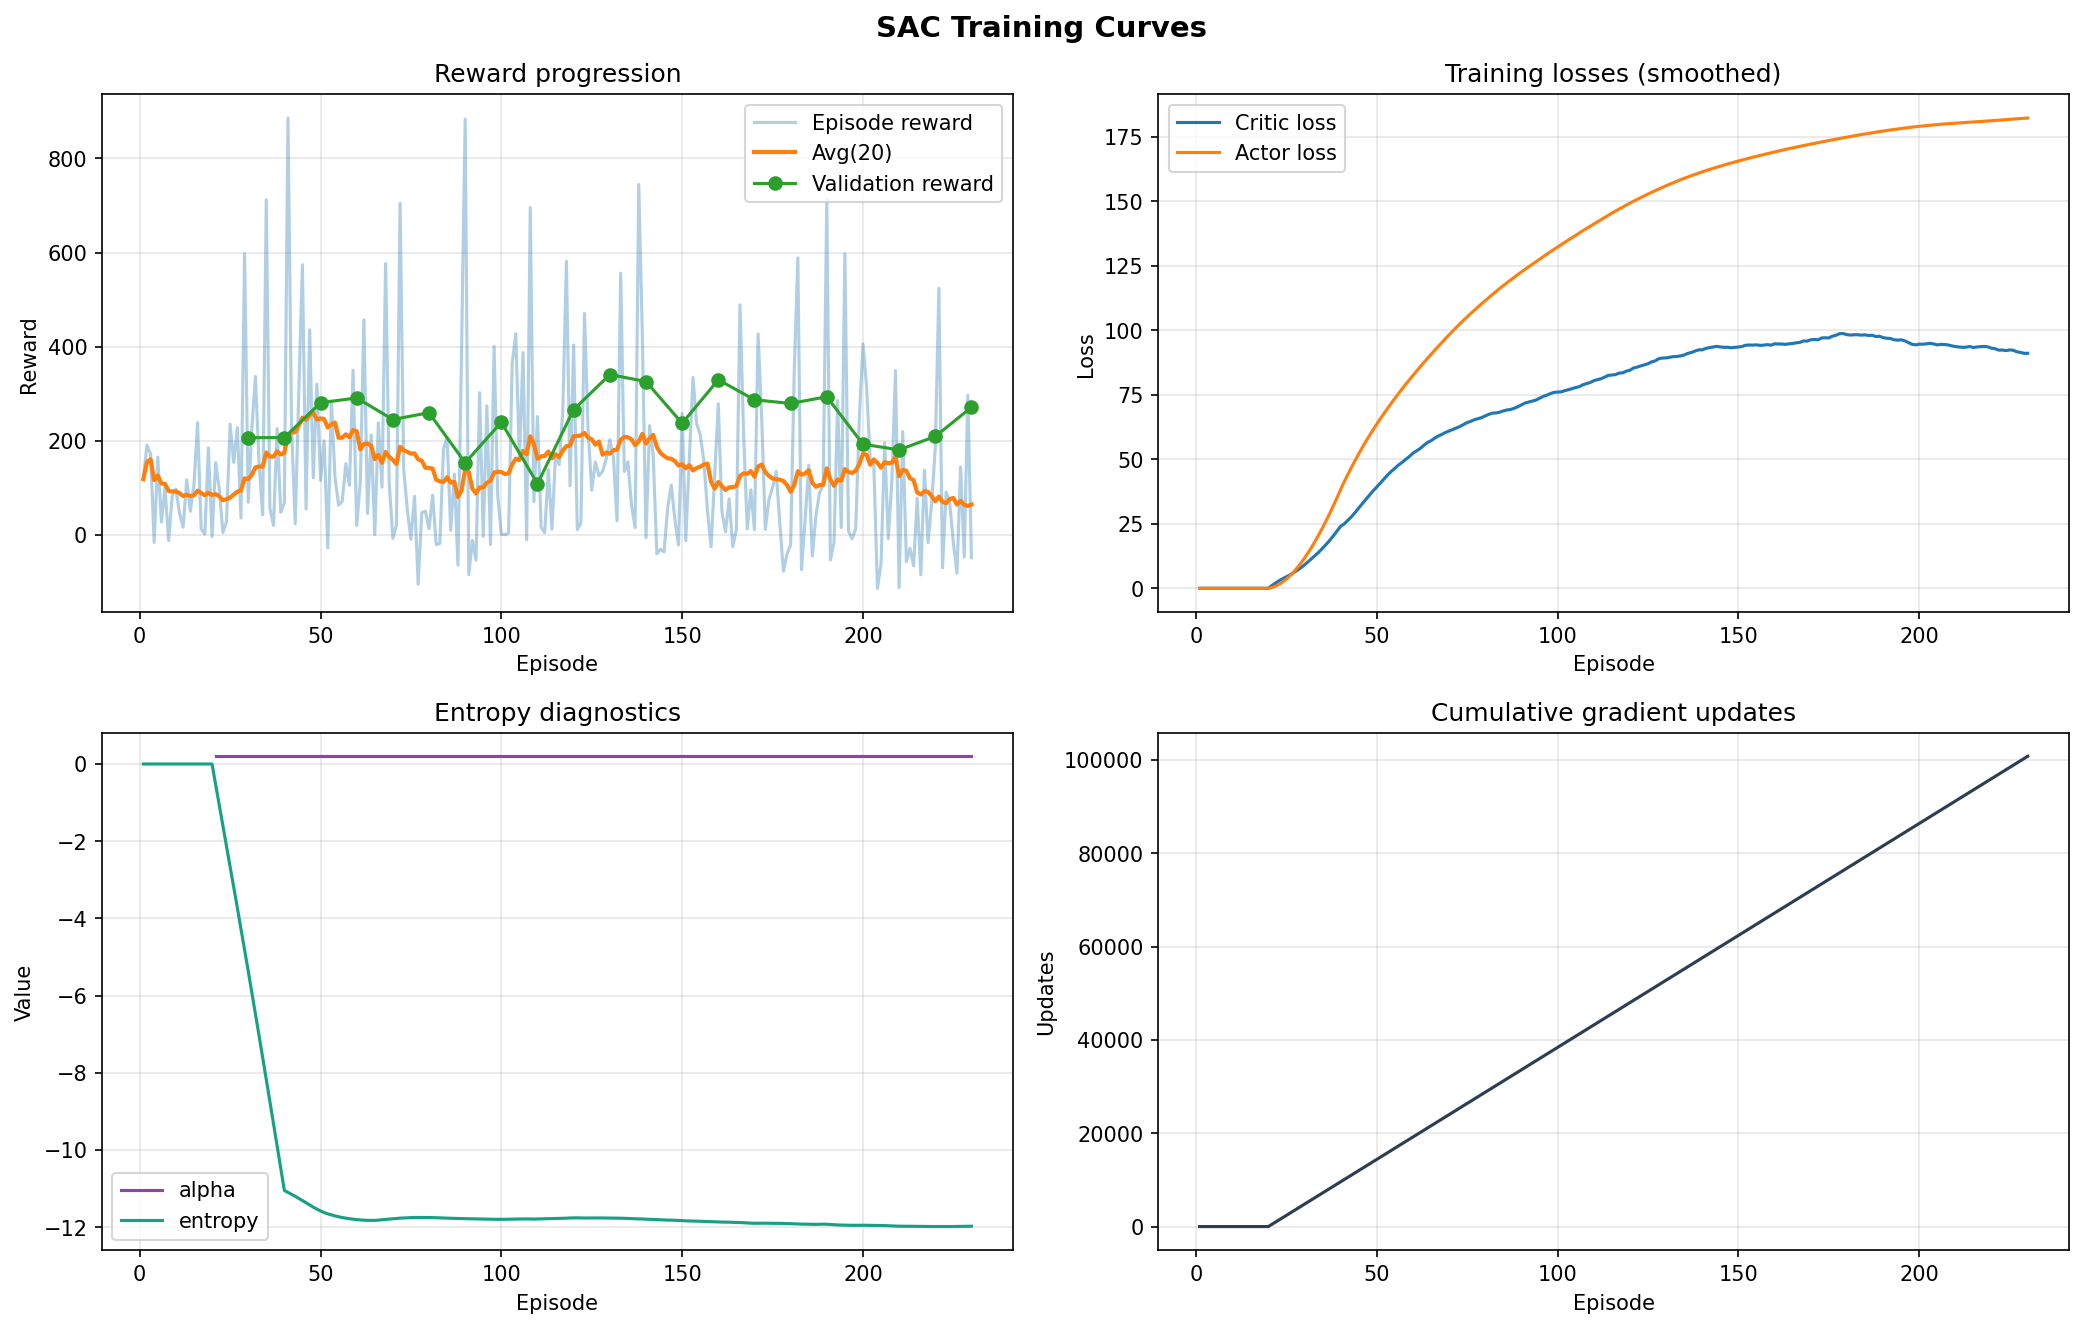
\includegraphics[width=0.75\textwidth]{figures/sac_train_curves.png}
    \caption{Courbes d'apprentissage SAC : reward par épisode,
             moyenne glissante (20), reward de validation,
             pertes critic/actor, entropie et mises à jour cumulées.
             Meilleur checkpoint à l'épisode~130
             (val reward 340.42), early stop épisode~230.}
    \label{fig:sac_train}
\end{figure}

\begin{figure}[H]
    \centering
    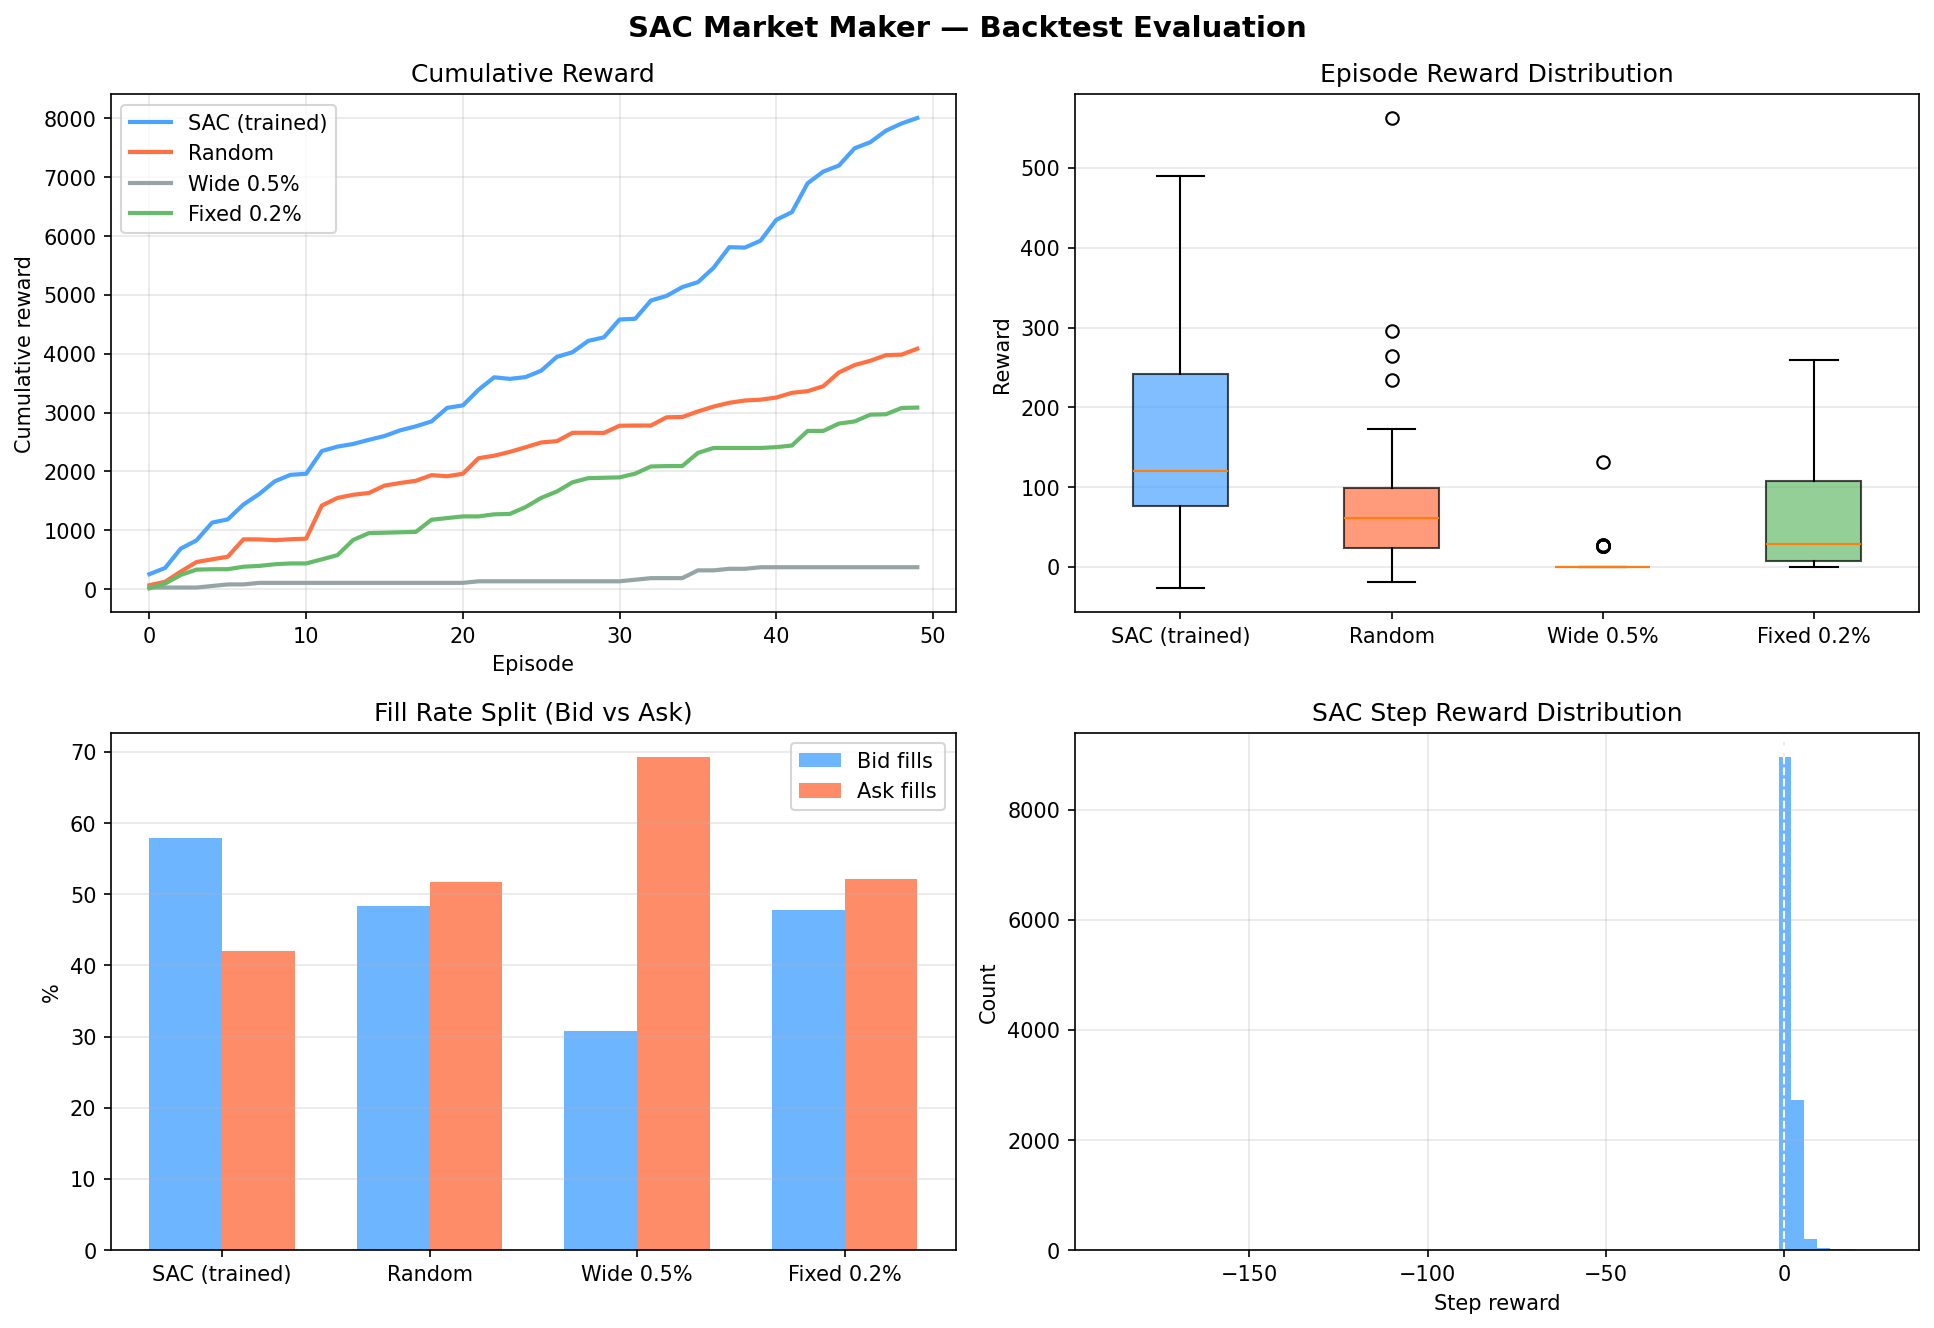
\includegraphics[width=0.75\textwidth]{figures/sac_eval.png}
    \caption{Évaluation multi-seed SAC (5 seeds $\times$ 50 épisodes) :
             reward cumulatif, distribution par épisode,
             taux de remplissage bid/ask et distribution des rewards par step.}
    \label{fig:sac_eval}
\end{figure}

\textbf{Entraînement.}
Hyperparamètres : LR~$= 3\times10^{-4}$, batch~256,
$\gamma = 0.99$, $\tau = 0.005$, 20 épisodes de warmup,
2 gradient steps par step d'environnement.
Le meilleur checkpoint est sauvegardé à l'épisode~130
(val reward~340.42) ; l'early stop se déclenche à
l'épisode~230 (patience de 100 épisodes sans amélioration),
soit moins de 10\% du budget total de 2\,500 épisodes.

\textbf{Évaluation multi-seed.}
Le meilleur checkpoint est évalué sur 5 seeds indépendantes
$\times$ 50 épisodes sur le jeu de test BTCUSDT
(15\% des données les plus récentes, jamais vues à
l'entraînement).

\begin{table}[H]
    \centering
    \begin{tabular}{l c c c c c}
        \toprule
        \textbf{Politique} & \textbf{Mean R} & \textbf{Sharpe}
            & \textbf{MaxDD} & \textbf{Fill\%} & \textbf{MaxInv} \\
        \midrule
        \textbf{SAC}  & $160.68 \pm 4.86$  & $8.82 \pm 0.82$
            & $7.09 \pm 10.15$ & $18.3 \pm 0.4$ & $1.49 \pm 0.07$ \\
        Random        & $84.92 \pm 14.16$  & $6.37 \pm 0.80$
            & $29.91 \pm 9.13$ & $7.2 \pm 0.6$  & $0.63 \pm 0.04$ \\
        Fixed 0.2\%   & $58.06 \pm 6.94$   & $4.62 \pm 0.99$
            & $0.00 \pm 0.00$  & $1.0 \pm 0.1$  & $0.18 \pm 0.02$ \\
        \bottomrule
    \end{tabular}
    \caption{Résultats SAC multi-seed vs baselines sur le jeu de test BTCUSDT.}
    \label{tab:sac_eval}
\end{table}

\textbf{Reward par épisode.}
La récompense de validation progresse rapidement dans les
130 premiers épisodes, atteignant un pic à 340.42. La
moyenne mobile sur 20 épisodes confirme cette tendance
haussière nette. Après l'épisode~130, le reward oscille
sans amélioration significative, ce qui déclenche l'early
stop à l'épisode~230 (patience de 100 épisodes). La
convergence en moins de 10\% du budget prévu de
2\,500 épisodes témoigne de l'efficacité de l'apprentissage
off-policy : le replay buffer permet de réutiliser les
expériences passées et d'apprendre plus rapidement qu'un
algorithme on-policy.

\textbf{Pertes critic et actor.}
La perte du critic se stabilise progressivement au fil de
l'entraînement, confirmant que les deux réseaux~$Q$
convergent vers des estimations cohérentes de la valeur
des paires (état, action). La perte de l'acteur est
décroissante en valeur absolue, signe que les Q-valeurs
estimées augmentent — comportement attendu d'une politique
qui s'améliore et apprend à citer des spreads mieux
positionnés. L'utilisation du minimum des deux critics
(clipped double-Q) contient efficacement la surestimation
qui affecte typiquement les algorithmes actor-critic.

\textbf{Entropie.}
Le coefficient $\alpha = 0.2$ reste constant comme prévu,
sans auto-tuning. La courbe d'entropie de la politique
s'effondre progressivement au cours de l'entraînement :
la politique devient quasi-déterministe. Pour un espace
d'action aussi contraint ($[0,\,0.5\%]^2$), ce comportement
est attendu et souhaitable — en inférence, une politique
déterministe est plus prévisible et plus facile à auditer.

\textbf{Évaluation multi-seed.}
Les 5 seeds indépendantes produisent des résultats
très cohérents (écart-type de 4.86 sur le mean reward
de 160.68), ce qui valide la stabilité de l'apprentissage
et l'absence de surapprentissage sur une graine particulière.
SAC surpasse systématiquement les deux baselines sur toutes
les métriques : $\times 2$ vs Random (84.92) et $\times 3$
vs Fixed~0.2\% (58.06). Le fill rate de 18.3\% montre que
l'agent a appris à citer de façon compétitive : suffisamment
proche du midprice pour être rempli fréquemment, tout en
capturant un spread suffisant pour être profitable. Le
Sharpe de 8.82 confirme que le rendement est obtenu avec
un risque maîtrisé. Le MaxDD de 7.09\% avec une variance
élevée ($\pm 10.15\%$) reflète la sensibilité aux conditions
de marché de la fenêtre de test, inhérente à tout agent
de market making face à un marché non stationnaire.

\subsection{Discussion}


\paragraph{Ce qui fonctionne.} Le moteur tient ses
objectifs de performance, l'intégration Binance est
stable, les stratégies par règles donnent une
\textit{baseline} interprétable et les agents RL
convergent sur les données d'entraînement.

\paragraph{Limites observées.} Les agents RL restent
sensibles à la qualité du \textit{reward shaping} et
à la non-stationnarité des marchés.

\paragraph{Pistes d'amélioration.}
\begin{itemize}[leftmargin=1.2cm]
    \item Enrichir l'espace d'état (carnet multi-niveaux,
          \textit{order flow imbalance}).
    \item Tester un \textit{reward} à risque ajusté
          (Sharpe différentiel).
    \item Intégrer un validation glissante sur données futures
          plus systématique.
\end{itemize}

% ===============================================================
\section{Manuel d'utilisation}
\label{sec:manuel}
% ===============================================================

\subsection{Pré-requis}

\begin{itemize}[leftmargin=1.2cm]
    \item CMake $\geq$ 3.10, compilateur C++20
          (GCC~10+, Clang~10+ ou MSVC~2019+).
    \item Python 3.10+, PyTorch
          (CUDA optionnel mais recommandé pour le DQN).
    \item Connexion Internet (API Binance, téléchargement
          des dépendances \texttt{libcurl} /
          \texttt{nlohmann/json}).
\end{itemize}

\subsection{Compilation}

\begin{lstlisting}[language=bash]
# Première fois (configuration initiale)
mkdir build && cd build
cmake ..
cmake --build . --config Release -j$(nproc)

# Builds suivants
./build.sh
\end{lstlisting}

\subsection{Lancement du moteur et des données live}

\begin{lstlisting}[language=bash]
# Tests + benchmarks
./build/OrderBookTests

# Affichage temps réel d'un symbole
./build/LiveMarketData SOLUSDT 1 20
# [SYMBOLE] [RAFRAICHISSEMENT_S] [PROFONDEUR]
\end{lstlisting}

\subsection{Lancement d'un agent}

\begin{lstlisting}[language=bash]
# Terminal 1 : flux de marché C++
./run_market.sh

# Terminal 2 : agent Python (stratégie au choix)
STRATEGY=mean_reversion python3 -m agents.main
STRATEGY=rsi             python3 -m agents.main
STRATEGY=bollinger       python3 -m agents.main
\end{lstlisting}

\subsection{Entraînement des agents RL}

\begin{lstlisting}[language=bash]
# DQN (variante normale)
python3 -m agents.train_dqn --variant normal \
    --csv BTCUSDT-aggTrades-2026-03.csv \
    --epochs 1 --rows-per-epoch 500000 \
    --warmup-rows 2000 --log-every 2000

# A2C
python3 -m agents.train_a2c

# Dreamer v3 (avec affichage live)
python3 run_dreamer.py
python3 run_dreamer.py --fast      # configuration CPU
\end{lstlisting}

\subsection{Tableau de bord}

\begin{lstlisting}[language=bash]
./run_dashboard.sh
# Puis ouvrir http://localhost:<port>/ dans le navigateur
\end{lstlisting}

\subsection{Configuration Binance testnet}

L'agent live utilise les clés API Binance testnet
définies dans \texttt{agents/exchange/config.py}
(à créer à partir de \texttt{config.example.py}).
Les clés peuvent être obtenues sur
\url{https://testnet.binance.vision/}.

% ===============================================================
\section{Maintenance}
\label{sec:maintenance}
% ===============================================================

\subsection{Mise à jour des dépendances}

\begin{itemize}[leftmargin=1.2cm]
    \item \textbf{C++} : les versions de \texttt{libcurl}
          et \texttt{nlohmann/json} sont fixées via
          \texttt{FetchContent} dans \texttt{CMakeLists.txt}.
          Mettre à jour les tags pour récupérer une nouvelle
          version, puis re-builder à blanc :
          \texttt{rm -rf build \&\& ./build.sh}.
    \item \textbf{Python} : \texttt{pip install -U torch
          numpy matplotlib pandas requests}.
\end{itemize}

\subsection{Ajout d'une nouvelle stratégie}

\begin{enumerate}[leftmargin=1.2cm]
    \item Créer \texttt{agents/strategies/ma\_strategie.py}
          implémentant l'interface \texttt{BaseStrategy}.
    \item L'enregistrer dans \texttt{agents/main.py}
          (branche \texttt{if strategy\_name == ...}).
    \item Tester via
          \texttt{STRATEGY=ma\_strategie python3 -m agents.main}.
\end{enumerate}

\subsection{Ré-entraînement périodique}

Les marchés évoluent : il est recommandé de
\textbf{ré-entraîner les agents RL} sur des données
récentes au moins une fois par mois, en vérifiant la
non-régression du PnL sur un jeu de validation
\textit{out-of-sample}.


% TODO: Compléter si une procédure de monitoring est
% mise en place (alertes Slack/mail, seuils de PnL, etc.)
\begin{itemize}[leftmargin=1.2cm]
    \item Lire les logs \texttt{dreamer\_train.log} et les
          CSV \texttt{dqn\_metrics/*.csv}.
    \item Surveiller la latence de l'API Binance.
    \item Conserver les checkpoints
          \texttt{models/*.pth} versionnés.
\end{itemize}

\subsection{Tests de non-régression}

\begin{lstlisting}[language=bash]
./build/OrderBookTests          # tests fonctionnels et perf C++
python3 test_dqn_manual.py      # validation actions DQN
python3 test_sma_manual.py      # validation SMA
python3 test_sac_state_manual.py # validation SAC state builder
\end{lstlisting}

\section{Conclusion}
\label{sec:conclusion}
% ===============================================================

Ce projet démontre la faisabilité d'une plateforme de
trading complète associant un \textbf{moteur de carnet
d'ordres en C++20 performant} ($O(\log n)$ insertion,
$O(1)$ annulation, latences microsecondes), une
\textbf{ingestion temps réel} de données Binance, une
\textbf{collection d'agents de trading} couvrant à la
fois les heuristiques classiques (mean reversion, RSI,
Bollinger) et les méthodes d'apprentissage par
renforcement modernes (DQN, A2C, PPO, SAC),
un \textbf{dashboard interactif} authentifié pour le monitoring
sans latence, et des \textbf{outils d'évaluation reproductibles}
(CSV, plots, multi-seed benchmarks).

Les expérimentations ont validé les exigences de
performance du moteur, ainsi que la convergence des
agents sur les jeux de données utilisés. L'agent SAC
en particulier démontre une capacité à surpasser les
baselines aléatoires et heuristiques sur le même dataset.
Les pistes d'extension naturelles concernent l'enrichissement de
l'espace d'état (\textit{order flow imbalance},
profondeur multi-niveaux), l'introduction de
\textit{rewards} à risque ajusté, et un protocole de
\textit{walk-forward validation} systématique pour
mieux capturer la non-stationnarité des marchés crypto.

\begin{thebibliography}{9}
\bibitem{dreamerv3} D. Hafner et al., \emph{Mastering Diverse Domains through World Models}, 2023.
\bibitem{sac} T. Haarnoja et al., \emph{Soft Actor-Critic: Off-Policy Deep Reinforcement Learning with a Stochastic Actor}, ICML, 2018.
\bibitem{ppo} J. Schulman et al., \emph{Proximal Policy Optimization Algorithms}, 2017.
\bibitem{ddqn} H. van Hasselt et al., \emph{Deep Reinforcement Learning with Double Q-learning}, AAAI, 2016.
\bibitem{gae} J. Schulman et al., \emph{High-Dimensional Continuous Control Using Generalized Advantage Estimation}, 2015.
\end{thebibliography}

\end{document}
